\documentclass[oneside]{article}
%DIF LATEXDIFF DIFFERENCE FILE
%DIF DEL method_validation_ms.tex             Mon Jan 24 14:20:58 2022
%DIF ADD method_validation_ms_revisions.tex   Mon Feb  7 14:17:19 2022

\usepackage{blindtext} % Package to generate dummy text throughout this template 
\usepackage{graphicx} % FKM: for figures
%DIF 5a5
\usepackage{wrapfig} %DIF > 
%DIF -------
\usepackage{color} % FKM: for colored text
\usepackage{float} % FKM: for forcing figure placement
\usepackage[breakable]{tcolorbox} % FKM: for text box
\usepackage{enumerate} % FKM: for bullet point lists
\usepackage{setspace} % FKM: line spacing
%DIF 10a11-13
\usepackage{soul} % strike through %DIF > 
\usepackage[normalem]{ulem} % strike through keeping emphasis standard %DIF > 
\usepackage{cancel} % diagonal strike through %DIF > 
%DIF -------
\usepackage[margin=1in]{geometry} % FKM: margins
%DIF 11-12d15
%DIF < 
%DIF < 
%DIF -------
\usepackage[sc]{mathpazo} % Use the Palatino font
\usepackage[T1]{fontenc} % Use 8-bit encoding that has 256 glyphs
% \linespread{1.05} % Line spacing - Palatino needs more space between lines
\usepackage{microtype} % Slightly tweak font spacing for aestheticsgins
\usepackage[small,labelfont=bf,up,up]{caption} % Custom captions under/above floats in tables or figures
\usepackage{booktabs} % Horizontal rules in tables
\usepackage{amsmath} % Text in equations
\usepackage{titlesec} % Allows customization of titles
\usepackage{titling} % Customizing the title section
\usepackage[hidelinks]{hyperref} % For hyperlinks in the PDF
%DIF 23a25
 %DIF > 
%DIF -------
\usepackage{tikz}
%DIF 24a27-30
\usepackage{bm} %DIF > 
\usepackage{scalefnt} %DIF > 
\usetikzlibrary{shapes.geometric, arrows, positioning, decorations.markings, shapes.multipart} %DIF > 
\usetikzlibrary{bayesnet} %DIF > 
%DIF -------
\usepackage{standalone}

%DIF 26a33-35
\usepackage{xr} % cross-referencing files %DIF > 
\externaldocument{method_validation_ms_supp} %DIF > 
 %DIF > 
%DIF -------
\usepackage{subcaption} % for subfigures side by side
\captionsetup[subfigure]{singlelinecheck=false} % to put (a) and (b) at the top-left of subfigures

\usepackage[shortlabels]{enumitem} % customized lists (shortlabels
                                % necessary to have i., ii., etc., in enumerate)
\setlist[itemize]{noitemsep} % Make itemize lists more compact

\usepackage{abstract} % Allows abstract customization
\renewcommand{\abstractnamefont}{\normalfont\bfseries} % Set the "Abstract" text to bold
\renewcommand{\abstracttextfont}{\normalfont\small\itshape} % Set the abstract itself to small italic text

\usepackage{fancyhdr} % Headers and footers
\pagestyle{fancy} % All pages have headers and footers
\fancyhead{} % Blank out the default header
\fancyfoot{} % Blank out the default footer
\fancyhead[C]{Authors et al. $\bullet$ August 2018 $\bullet$ bio{\color{red}R}$\chi$ve} % Custom header text
\fancyfoot[RO,LE]{\thepage} % Custom footer text



\usepackage{natbib}
\bibliographystyle{apalike}

\usepackage{libertine}

\setlength\columnsep{20pt}

%----------------------------------------------------------------------------------------
%	TITLE SECTION
%----------------------------------------------------------------------------------------

\setlength{\droptitle}{-4\baselineskip} % Move the title up

%\pretitle{\begin{center}\Huge\bfseries} % Article title formatting
%\posttitle{\end{center}} % Article title closing formatting

\title{How to validate a Bayesian model} % Article title
%DIF 63a73-74
%LM: strictly speaking, we're 'validating' the inference machinery. %DIF > 
%% Validating a model involves epistemic considerations that are, as far as I understand, outside the scope of this paper. %DIF > 
%DIF -------
\author{\textsc{F\'{a}bio K. Mendes\DIFdelbegin \DIFdel{$^{1*}$}\DIFdelend \DIFaddbegin \DIFadd{$^{1\dagger}$}\DIFaddend }, \textsc{Remco Bouckaert\DIFdelbegin \DIFdel{$^{2*}$}\DIFdelend \DIFaddbegin \DIFadd{$^{2\dagger*}$}\DIFaddend },\\
\textsc{\DIFdelbegin \DIFdel{Christiaan Swanepoel$^{2}$}\DIFdelend \DIFaddbegin \DIFadd{Luiz M. Carvalho$^{3\dagger}$}\DIFaddend }, \textsc{Alexei J. Drummond\DIFdelbegin \DIFdel{$^{1,2}$}\DIFdelend \DIFaddbegin \DIFadd{$^{4}$}\DIFaddend } \\
\small $^1$\DIFdelbegin \DIFdel{School of Biological Sciences}\DIFdelend \DIFaddbegin \DIFadd{Department of Biology, Washington University in St. Louis}\\
\small \DIFadd{$^2$School of Computer Science}\DIFaddend , The University of Auckland\\
\small \DIFdelbegin \DIFdel{$^2$School of Computer Science}\DIFdelend \DIFaddbegin \DIFadd{$^3$Escola de Matem\'{a}tica Aplicada, Fundaç\~{a}o Get\'{u}lio Vargas}\\
\small \DIFadd{$^4$School of Biological Sciences}\DIFaddend , The University of Auckland\\
\small
\href{mailto:f.mendes@auckland.ac.nz}{\DIFaddbegin \DIFadd{$^*$}\DIFaddend Corresponding authors\DIFdelbegin \DIFdel{$^*$}\DIFdelend :
  f.mendes@auckland.ac.nz\DIFdelbegin \DIFdel{, }\DIFdelend \DIFaddbegin \DIFadd{; }\DIFaddend remco@cs.auckland.ac.nz}\DIFaddbegin \\
{\small \DIFadd{$^\dagger$Authors contributed equally to this work}}
\DIFaddend % \href{mailto:f.mendes@auckland.ac.nz}{another.email@auckland.ac.nz}
%\and % Uncomment if 2 authors are required, duplicate these 4 lines if more
%\textsc{Jane Smith}\thanks{Corresponding author} \\[1ex] % Second author's name
%\normalsize University of Utah \\ % Second author's institution
%\normalsize \href{mailto:jane@smith.com}{jane@smith.com} % Second author's email address
}
\date{\today} % Leave empty to omit a date
\renewcommand{\maketitlehookd}{%
\begin{abstract}
  \noindent Biology has become a highly mathematical discipline in
  which probabilistic models play a central role,
  and as a result research in the biological sciences is now dependent on
  computational tools capable of carrying out complex analyses.
  These tools must not only be efficient, but also correctly
  implemented.
  Both goals are difficult to achieve for several reasons, such as the
  multidisciplinary nature of method development, and a still
  embrionic literature on good software development and statistical
  practices aimed at professionals from disparate fields.
  Here we provide guidelines for the validation of probabilistic model
  implementations, focusing on Bayesian approaches.
  This manuscript summarizes good practices for assessing the correctness of
  simulation and inference procedures under a model, and is available in
  the traditionally static print version as well as in a reproducible and
  executable form.
\end{abstract}
\centering [Probabilistic models, Bayesian models, model validation, coverage]
}

%----------------------------------------------------------------------------------------

\doublespacing
%DIF PREAMBLE EXTENSION ADDED BY LATEXDIFF
%DIF UNDERLINE PREAMBLE %DIF PREAMBLE
\RequirePackage[normalem]{ulem} %DIF PREAMBLE
\RequirePackage{color}\definecolor{RED}{rgb}{1,0,0}\definecolor{BLUE}{rgb}{0,0,1} %DIF PREAMBLE
\providecommand{\DIFaddtex}[1]{{\protect\color{blue}\uwave{#1}}} %DIF PREAMBLE
\providecommand{\DIFdeltex}[1]{{\protect\color{red}\sout{#1}}}                      %DIF PREAMBLE
%DIF SAFE PREAMBLE %DIF PREAMBLE
\providecommand{\DIFaddbegin}{} %DIF PREAMBLE
\providecommand{\DIFaddend}{} %DIF PREAMBLE
\providecommand{\DIFdelbegin}{} %DIF PREAMBLE
\providecommand{\DIFdelend}{} %DIF PREAMBLE
\providecommand{\DIFmodbegin}{} %DIF PREAMBLE
\providecommand{\DIFmodend}{} %DIF PREAMBLE
%DIF FLOATSAFE PREAMBLE %DIF PREAMBLE
\providecommand{\DIFaddFL}[1]{\DIFadd{#1}} %DIF PREAMBLE
\providecommand{\DIFdelFL}[1]{\DIFdel{#1}} %DIF PREAMBLE
\providecommand{\DIFaddbeginFL}{} %DIF PREAMBLE
\providecommand{\DIFaddendFL}{} %DIF PREAMBLE
\providecommand{\DIFdelbeginFL}{} %DIF PREAMBLE
\providecommand{\DIFdelendFL}{} %DIF PREAMBLE
%DIF HYPERREF PREAMBLE %DIF PREAMBLE
\providecommand{\DIFadd}[1]{\texorpdfstring{\DIFaddtex{#1}}{#1}} %DIF PREAMBLE
\providecommand{\DIFdel}[1]{\texorpdfstring{\DIFdeltex{#1}}{}} %DIF PREAMBLE
\newcommand{\DIFscaledelfig}{0.5}
%DIF HIGHLIGHTGRAPHICS PREAMBLE %DIF PREAMBLE
\RequirePackage{settobox} %DIF PREAMBLE
\RequirePackage{letltxmacro} %DIF PREAMBLE
\newsavebox{\DIFdelgraphicsbox} %DIF PREAMBLE
\newlength{\DIFdelgraphicswidth} %DIF PREAMBLE
\newlength{\DIFdelgraphicsheight} %DIF PREAMBLE
% store original definition of \includegraphics %DIF PREAMBLE
\LetLtxMacro{\DIFOincludegraphics}{\includegraphics} %DIF PREAMBLE
\newcommand{\DIFaddincludegraphics}[2][]{{\color{blue}\fbox{\DIFOincludegraphics[#1]{#2}}}} %DIF PREAMBLE
\newcommand{\DIFdelincludegraphics}[2][]{% %DIF PREAMBLE
\sbox{\DIFdelgraphicsbox}{\DIFOincludegraphics[#1]{#2}}% %DIF PREAMBLE
\settoboxwidth{\DIFdelgraphicswidth}{\DIFdelgraphicsbox} %DIF PREAMBLE
\settoboxtotalheight{\DIFdelgraphicsheight}{\DIFdelgraphicsbox} %DIF PREAMBLE
\scalebox{\DIFscaledelfig}{% %DIF PREAMBLE
\parbox[b]{\DIFdelgraphicswidth}{\usebox{\DIFdelgraphicsbox}\\[-\baselineskip] \rule{\DIFdelgraphicswidth}{0em}}\llap{\resizebox{\DIFdelgraphicswidth}{\DIFdelgraphicsheight}{% %DIF PREAMBLE
\setlength{\unitlength}{\DIFdelgraphicswidth}% %DIF PREAMBLE
\begin{picture}(1,1)% %DIF PREAMBLE
\thicklines\linethickness{2pt} %DIF PREAMBLE
{\color[rgb]{1,0,0}\put(0,0){\framebox(1,1){}}}% %DIF PREAMBLE
{\color[rgb]{1,0,0}\put(0,0){\line( 1,1){1}}}% %DIF PREAMBLE
{\color[rgb]{1,0,0}\put(0,1){\line(1,-1){1}}}% %DIF PREAMBLE
\end{picture}% %DIF PREAMBLE
}\hspace*{3pt}}} %DIF PREAMBLE
} %DIF PREAMBLE
\LetLtxMacro{\DIFOaddbegin}{\DIFaddbegin} %DIF PREAMBLE
\LetLtxMacro{\DIFOaddend}{\DIFaddend} %DIF PREAMBLE
\LetLtxMacro{\DIFOdelbegin}{\DIFdelbegin} %DIF PREAMBLE
\LetLtxMacro{\DIFOdelend}{\DIFdelend} %DIF PREAMBLE
\DeclareRobustCommand{\DIFaddbegin}{\DIFOaddbegin \let\includegraphics\DIFaddincludegraphics} %DIF PREAMBLE
\DeclareRobustCommand{\DIFaddend}{\DIFOaddend \let\includegraphics\DIFOincludegraphics} %DIF PREAMBLE
\DeclareRobustCommand{\DIFdelbegin}{\DIFOdelbegin \let\includegraphics\DIFdelincludegraphics} %DIF PREAMBLE
\DeclareRobustCommand{\DIFdelend}{\DIFOaddend \let\includegraphics\DIFOincludegraphics} %DIF PREAMBLE
\LetLtxMacro{\DIFOaddbeginFL}{\DIFaddbeginFL} %DIF PREAMBLE
\LetLtxMacro{\DIFOaddendFL}{\DIFaddendFL} %DIF PREAMBLE
\LetLtxMacro{\DIFOdelbeginFL}{\DIFdelbeginFL} %DIF PREAMBLE
\LetLtxMacro{\DIFOdelendFL}{\DIFdelendFL} %DIF PREAMBLE
\DeclareRobustCommand{\DIFaddbeginFL}{\DIFOaddbeginFL \let\includegraphics\DIFaddincludegraphics} %DIF PREAMBLE
\DeclareRobustCommand{\DIFaddendFL}{\DIFOaddendFL \let\includegraphics\DIFOincludegraphics} %DIF PREAMBLE
\DeclareRobustCommand{\DIFdelbeginFL}{\DIFOdelbeginFL \let\includegraphics\DIFdelincludegraphics} %DIF PREAMBLE
\DeclareRobustCommand{\DIFdelendFL}{\DIFOaddendFL \let\includegraphics\DIFOincludegraphics} %DIF PREAMBLE
%DIF LISTINGS PREAMBLE %DIF PREAMBLE
\RequirePackage{listings} %DIF PREAMBLE
\RequirePackage{color} %DIF PREAMBLE
\lstdefinelanguage{DIFcode}{ %DIF PREAMBLE
%DIF DIFCODE_UNDERLINE %DIF PREAMBLE
  moredelim=[il][\color{red}\sout]{\%DIF\ <\ }, %DIF PREAMBLE
  moredelim=[il][\color{blue}\uwave]{\%DIF\ >\ } %DIF PREAMBLE
} %DIF PREAMBLE
\lstdefinestyle{DIFverbatimstyle}{ %DIF PREAMBLE
	language=DIFcode, %DIF PREAMBLE
	basicstyle=\ttfamily, %DIF PREAMBLE
	columns=fullflexible, %DIF PREAMBLE
	keepspaces=true %DIF PREAMBLE
} %DIF PREAMBLE
\lstnewenvironment{DIFverbatim}{\lstset{style=DIFverbatimstyle}}{} %DIF PREAMBLE
\lstnewenvironment{DIFverbatim*}{\lstset{style=DIFverbatimstyle,showspaces=true}}{} %DIF PREAMBLE
%DIF END PREAMBLE EXTENSION ADDED BY LATEXDIFF

\begin{document}

% Print the title
\maketitle

%----------------------------------------------------------------------------------------
%	ARTICLE CONTENTS
%----------------------------------------------------------------------------------------

\section*{Introduction}
The last two decades have seen the biological sciences undergo a major revolution.
Critical technological innovations such as the advent of massive
parallel sequencing and the accompanying improvements in computational
power and storage have flooded biology with unprecedented amounts of
data ripe for analysis.
Not only has intraspecific data from multiple individuals allowed
progress in fields like medicine and epidemiology
\citep[e.g.,][]{1000g,humanmicrobiome,neafsey15}, population genetics
\citep[e.g.,][]{lynch07,lack16,demanuel16} and disease ecology
\citep[e.g.,][]{rosenblum13,bates18}, but now a large number of species
across the tree of life have had their genomes sequenced, furthering
our understanding of species relationships and diversification
\citep[e.g.,][]{martin13,brawand14,jarvis14,novikova16,pease2016,kawahara19,upham19}.
However, as the old adage goes, with great power comes great
responsibility: never has the data available to the average biologist
been so abundant, but also never has one been so aware of both its
complexity and the necessary care needed to analyze it.
Almost on par with with data accumulation is the rate at which new
computational tools are being proposed, as evidenced by journals
entirely dedicated to method advances, methodological sections in
biological journals, and computational biology degrees being offered
by institutions around the world.

One extreme case is the discipline of evolutionary biology (on which
we focus our attention).
While it could be said that many decade-old questions and hypotheses
in evolutionary biology have aged well and stood up the test of time
(e.g., the Red Queen hypothesis,
\citealt{vanvalen73,lively87,morran11,gibson15}; the
Bateson-Dobzhansky-Muller model,
\citealt{dob36,muller40,hopkins12,roda17}), data analysis practices
have changed drastically in recent years, to the point they would
likely seem exotic and obscure to an evolutionary biologist active
forty years ago.
In particular, evolutionary biology has become highly statistical,
with the development and utilization of models now being commonplace.

Models are employed in the sciences for many reasons, and fall within
a biological abstraction continuum \citep{servedio14}, going from
fully verbal, highly abstract models (e.g., \citealt{vanvalen73}),
through proof-of-concept models that formalize verbal models (e.g.,
\citealt{maynard78,reinhold99,mendes18}), to models that
interact directly with data through explicit mathematical
functions \citep{yule24,felsenstein73,hky,hudson90}\DIFdelbegin \DIFdel{)}\DIFdelend .
Within the latter category, probabilistic models have seen a sharp surge
in popularity within evolutionary biology, in conjunction
with computational tools implementing them.

Despite the increasing pervasiveness of probabilistic models in the
biological sciences, tools implementing such models show large
variation not only with respect to code quality (from a software engineering
perspective), but also correctness \citep{darriba18}.
This is unsurprising given the multidisciplinary nature of model and method
development, and the challenges inherent to software research funding
\citep{siepel19}.
The bioinformatics community is thus in dire need of resources that
provide guidance for code improvement and validation.

Here, we summarize best practices in probabilistic model validation for method
developers, with an emphasis on Bayesian methods.
\DIFdelbegin \DIFdel{This manuscript is also presented in a reproducible and executable version
}%DIFDELCMD < [%%%
\DIFdel{LINK TO STENCILA VERSION}%DIFDELCMD < ]%%%
\DIFdel{, and is accompanied by code examples for these practices
(with }\DIFdelend \DIFaddbegin \DIFadd{Scripts for reproducing our validation protocols and figures are available on
\textcolor{red}{[Link to DeveloperManual]}.
This repository also hosts tools for model validation within }\DIFaddend the BEAST 2 platform
\DIFdelbegin \DIFdel{as a reference; \mbox{%DIFAUXCMD
\citealp{beast25}}\hspace{0pt}%DIFAUXCMD
)}\DIFdelend \DIFaddbegin \DIFadd{\mbox{%DIFAUXCMD
\citep{beast25}}\hspace{0pt}%DIFAUXCMD
}\DIFaddend .

% \begin{figure}
%   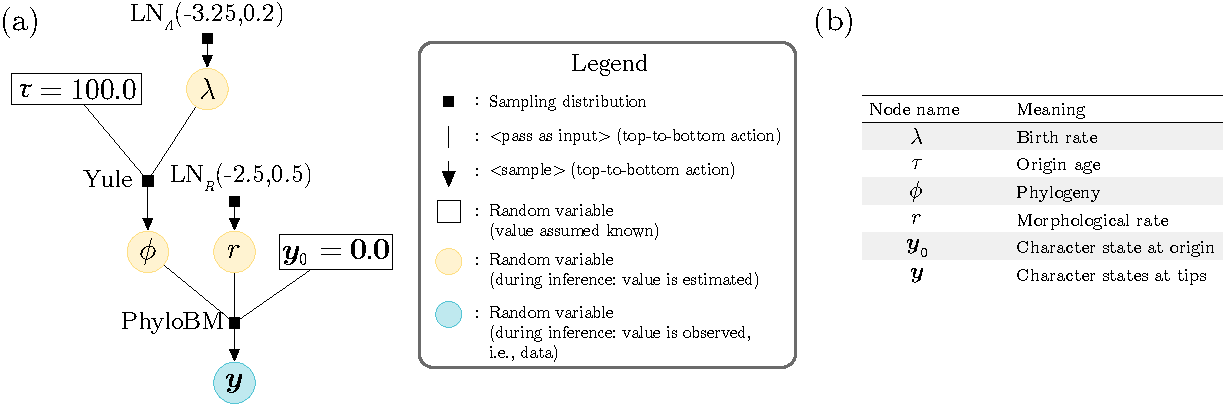
\includegraphics[width=\linewidth]{fig1}
%   \caption{Hemiplasy on species trees and gene trees.
%     Panel (a) shows substitutions that occur on each of the two discordant gene trees, and the corresponding site patterns produced.
%     (b) Incorrectly inferred convergent substitutions (from the site patterns produced in [a]) when analyses are conducted on the species tree topology.
%     (c) Incorrectly inferred convergent substitutions when analyses are conducted on the CDS tree (discordant tree topology 2).}
%   \label{fig:1}
% \end{figure}

%------------------------------------------------

\section*{Probabilistic models}

Probabilistic models mathematically formalize natural phenomena
having an element of randomness.
This is done through probability distributions describing both the observed
empirical data -- seen as the result of one or more random
instantiations of the modeled process -- as well the model parameters,
which abstract relevant, but usually unknown aspects
of the phenomenon at hand.
The historical, stochastic, and highly dimensional nature of evolutionary
processes makes the utility of probabilistic models in evolutionary
biology self-evident. 

The central component of a probabilistic model, \DIFdelbegin \DIFdel{$\text{P}(D|\theta)$,
describes }\DIFdelend \DIFaddbegin \DIFadd{$\text{Pr}(D=d|\Theta=\theta)$,
allows us to describe }\DIFaddend the probability distribution over the data \DIFaddbegin \DIFadd{($d$) }\DIFaddend given the model
parameters \DIFaddbegin \DIFadd{($\theta$)}\DIFaddend .
This probability mass function (pmf; or its continuous
countepart, the probability density function\DIFdelbegin \DIFdel{$f(D|\theta)$}\DIFdelend \DIFaddbegin \DIFadd{, pdf, $f_D(d|\Theta=\theta)$}\DIFaddend ) is sometimes
referred to as the likelihood function.
\DIFaddbegin \DIFadd{(We will henceforth simplify notation and drop variable subscripts, e.g., $f_D(d|\Theta=\theta) \rightarrow f(d|\theta)$,
and also assume variables are always continuous).
}\DIFaddend As illustrated in the next sections, probabilistic models can be
hierarchical, in which case there may be several likelihood functions.
% (Fig. \ref{fig:graphmodel}).
In a frequentist statistical framework, \DIFdelbegin \DIFdel{$\text{P}(D|\theta)$ }\DIFdelend \DIFaddbegin \DIFadd{$f(d|\theta)$ }\DIFaddend is the sole
component of a probabilistic model, and is maximized across parameter \DIFdelbegin \DIFdel{($\theta$) }\DIFdelend space during
parameter estimation and model comparison.

In the present study we focus on Bayesian inference, however, 
where a probabilistic model $\mathcal{M}$ defines a posterior probability
distribution for its parameters, \DIFdelbegin \DIFdel{$\text{P}(\theta|D) =
\frac{\text{P}(D|\theta)\text{P}(\theta)}{\text{P}(D)}$}\DIFdelend \DIFaddbegin \DIFadd{$f(\theta|d) =
\frac{f(d|\theta)f(\theta)}{f(d)}$}\DIFaddend .
Here, our prior inferences or beliefs about the natural world -- represented by
the prior distribution \DIFdelbegin \DIFdel{$\text{P}(\theta)$ }\DIFdelend \DIFaddbegin \DIFadd{$f(\theta)$ }\DIFaddend -- are confronted and updated by
the data through the likelihood function (or multiple likelihood functions).
\DIFdelbegin \DIFdel{$\text{P}(D) = \int_\theta \text{P}(D|\theta)\text{P}(\theta)d\theta$}\DIFdelend \DIFaddbegin \DIFadd{$f(d) = \int_\Theta f(d|\theta)f(\theta)d\theta$}\DIFaddend , the
probability of the data, is also known as the marginal likelihood or the model
evidence.
Crucially, a Bayesian model includes a prior, \DIFdelbegin \DIFdel{$\text{P}(\theta)$}\DIFdelend \DIFaddbegin \DIFadd{$f(\theta)$}\DIFaddend :
when models are compared, for example, \DIFdelbegin \DIFdel{$\text{P}(\theta)$ }\DIFdelend \DIFaddbegin \DIFadd{$f(\theta)$ }\DIFaddend needs to be taken
into account when computing the model evidence \DIFdelbegin \DIFdel{$\text{P}(D)$}\DIFdelend \DIFaddbegin \DIFadd{$f(d)$}\DIFaddend .

Models routinely used in evolutionary biology are often characterized by
continuous parameters, and are normally complex enough to preclude
analytical solutions for the posterior density \DIFdelbegin \DIFdel{$f(\theta|D)$}\DIFdelend \DIFaddbegin \DIFadd{$f(\theta|d)$}\DIFaddend , mainly
due to the intractability of the integral appearing in the marginal
likelihood.
In those cases, one can make use of the fact that \DIFdelbegin \DIFdel{$f(D)$
}\DIFdelend \DIFaddbegin \DIFadd{$f(d)$
}\DIFaddend is a constant that can be ignored (i.e., \DIFdelbegin \DIFdel{$f(\theta|D)
\propto f(\theta|D)f(\theta)$}\DIFdelend \DIFaddbegin \DIFadd{$f(\theta|d)
\propto f(\theta|d)f(\theta)$}\DIFaddend ), and use 
techniques like Markov chain Monte Carlo (MCMC) to sample the posterior
distribution.
This is because the MCMC algorithm that generates the Markov chain,
called the Metropolis-Hastings \citep{metropolis53,mh} algorithm, only requires the
posterior to be evaluated up to a constant.

In practice, the Metropolis-Hastings algorithm samples the posterior
distribution (also referred to as the ``target'' distribution) by means of a
transition mechanism. 
If the proposal distribution generated by this mechanism is
irreducible, positive recurrent, and aperiodic, and the resulting
chain is long enough, then the sampled posterior distribution will approximate
the target distribution \DIFdelbegin \DIFdel{$f(\theta|D)$ }\DIFdelend \DIFaddbegin \DIFadd{$f(\theta|d)$ }\DIFaddend \citep{smith93,tierney94,gelman}.

We will spend time considering MCMC in particular as it is the commonly
chosen technique for obtaining \DIFdelbegin \DIFdel{$f(\theta|D)$ }\DIFdelend \DIFaddbegin \DIFadd{$f(\theta|d)$ }\DIFaddend under an implementation of
model $\mathcal{M}$.
A thorough validation effort thus entails verifying the
correctness of (i) the model (i.e., \DIFdelbegin \DIFdel{$f(D|\theta)f(\theta)$}\DIFdelend \DIFaddbegin \DIFadd{$f(d|\theta)f(\theta)$}\DIFaddend ), and (ii)
the components involved in the MCMC transition mechanism.
We note that the latter are not part of the model, however, and it is 
possible to sample \DIFdelbegin \DIFdel{$f(\theta|D)$ }\DIFdelend \DIFaddbegin \DIFadd{$f(\theta|d)$ }\DIFaddend with other techniques such as importance
sampling, Hamiltonian Monte Carlo \citep{hmc}, or even by converting the
sampling problem into an optimization one \citep[e.g.,][]{zhang18}.

Finally, we stress that we are interested in practices for verifying model
\emph{correctness}.
There are other tests employed to ensure that a particular MCMC analysis
is converging as anticipated.
Determining that one or more independent Markov chains converged on very
similar posterior distributions is not a correctness test, as those
distributions might be very different from the target distribution.

\subsection*{Validating a Bayesian model}

\subsubsection*{Validating the simulator, \DIFdelbegin \DIFdel{$S[\mathcal{M}]$}\DIFdelend \DIFaddbegin \DIFadd{$\text{S}[\mathcal{M}]$}\DIFaddend }
\label{verify-correctness-of-simulator-implementation}

When a probabilistic model $\mathcal{M}$ is implemented for the first
time, a simulator \DIFdelbegin \DIFdel{$S[\mathcal{M}]$ }\DIFdelend \DIFaddbegin \DIFadd{$\text{S}[\mathcal{M}]$ }\DIFaddend must be devised and itself
validated before we can validate an inferential engine \DIFdelbegin \DIFdel{$I[\mathcal{M}]$}\DIFdelend \DIFaddbegin \DIFadd{$\text{I}[\mathcal{M}]$}\DIFaddend .
It is \DIFdelbegin \DIFdel{$I[\mathcal{M}]$ }\DIFdelend \DIFaddbegin \DIFadd{$\text{I}[\mathcal{M}]$ }\DIFaddend that will be employed by users in empirical
analyses.
\DIFaddbegin \begin{wrapfigure}{l}{5.5cm}
  \includestandalone[width=5.75cm]{../figures/graphical_model}    
  \caption{\DIFadd{The graphical representation of a simple Bayesian
    phylogenetic model.
    Parameters are represented by yellow circles, observed data
    in blue circles, and fixed values are shown within boxes.
    Sampling distributions are represented by filled squares.
    LN($\mu,\sigma^2$) denote log-normal sampling distributions
    with mean $\mu$ and variance $\sigma^2$ in log-space.
    Parameter descriptions can be found in the main text.
    }}
  \label{fig:pgm}
\end{wrapfigure}
\DIFaddend A simulator conventionally requires a parameter value as input (i.e.,
a $\theta$ value, where $\boldsymbol{\theta}$ might represent more than one
parameter), or a prior distribution on those values,
$f(\boldsymbol{\theta})$. 
The simulator then outputs a sample of random variable(s), which
for hierarchical models will include not only an instantiation of data
$\text{D}$, but also of a subset of the parameters in
$\boldsymbol{\theta}$.

In the case of hierarchical models, it is sometimes useful
to consider \DIFdelbegin \DIFdel{$S[\mathcal{M}]$ }\DIFdelend \DIFaddbegin \DIFadd{$\text{S}[\mathcal{M}]$ }\DIFaddend as a collection of component
simulators, each characterized by a different sampling distribution.
In figure X, for example, \DIFdelbegin \DIFdel{$S[\mathcal{M}]$ }\DIFdelend \DIFaddbegin \DIFadd{$\text{S}[\mathcal{M}]$ }\DIFaddend can be seen as an ensemble
comprised by (i) \DIFdelbegin \DIFdel{$S[f(\boldsymbol{\theta})]$ (where $\boldsymbol{\theta} = \{\lambda, r, r_m,
y_0\}$}\DIFdelend \DIFaddbegin \DIFadd{$\text{S}[f(\boldsymbol{\theta})]$ (where $\boldsymbol{\theta} = \{\lambda, r, y_0\}$}\DIFaddend ),
which jointly simulates all parameters in $\boldsymbol{\theta}$,
(ii) \DIFdelbegin \DIFdel{$S[f(\Phi|\lambda)]$}\DIFdelend \DIFaddbegin \DIFadd{$\text{S}[f(\Phi|\lambda)]$}\DIFaddend , which simulates a Yule tree $\Phi$ \DIFdelbegin \DIFdel{, (}\DIFdelend \DIFaddbegin \DIFadd{given a
value of $\lambda$ simulated in (i), and (}\DIFaddend iii)
\DIFdelbegin \DIFdel{$S[f(\mathbf{A}|\Phi,r)]$, which simulates a multiple sequence
alignment $\mathbf{A}$, and (iv)
$S[f(\mathbf{M}|\Phi,r_m,y_0])$}\DIFdelend \DIFaddbegin \DIFadd{$\text{S}[f(\boldsymbol{y}|\Phi,r)]$}\DIFaddend , which simulates \DIFdelbegin \DIFdel{a continuous character vector $\mathbf{M}$ for all
species in }\DIFdelend \DIFaddbegin \DIFadd{an array of $n$ continuous-trait
values, $\boldsymbol{y}$, given a phylogeny }\DIFaddend $\Phi$ \DIFaddbegin \DIFadd{with $n$ species and
an evolutionary rate $r$ (simulated in }[\DIFadd{i}] \DIFadd{and }[\DIFadd{ii}]\DIFadd{, respectively)}\DIFaddend .
Being able to isolate the building blocks of a hierarchical model simulator 
helps divide and conquer the validation task, especially when some, but
not all of the sampling distributions are well-known parametric distributions,
or when they result from well characterized stochastic processes (see below).

One way \DIFdelbegin \DIFdel{of validating }\DIFdelend \DIFaddbegin \DIFadd{to validate }\DIFaddend a probabilistic model simulator is by
\DIFdelbegin \DIFdel{sampling }\DIFdelend \DIFaddbegin \DIFadd{using it to sample }\DIFaddend a large number of \DIFdelbegin \DIFdel{points, calculating summary statistics
from the sample, and comparing those statistics to either their true value
counterparts (i.
e., the values used as input in the simulation), or to their analytical expectations.
In Box 1, we illustrate this procedure for a known parametric distribution, the
multivariate normal distribution characterizing the phylogenetic
Brownian motion model \mbox{%DIFAUXCMD
\citep{felsenstein73}}\hspace{0pt}%DIFAUXCMD
.
}\DIFdelend \DIFaddbegin \DIFadd{data sets given a set of parameters.
These parameters can be seen as characterizing a ``population''
of the entities being modeled.
For each data set, one can then construct $\alpha$-confidence intervals
(where $\alpha \in (0,1)$ gives the credibility level) for
certain summary statistics
(e.g., mean, variance, covariance).
If the simulator is behaving as expected, one should
be able to verify that the (population) summary statistic
is contained approximately $\alpha$\% of the time within their
$\alpha$-confidence intervals.
An example is the Yule model (also known as the pure-birth model;
\mbox{%DIFAUXCMD
\citealt{yule24}}\hspace{0pt}%DIFAUXCMD
), a continuous-time Markov process that has been
classically employed in phylogenetics to model the number of
species in a clade \mbox{%DIFAUXCMD
\citep{yule24,aldous01}}\hspace{0pt}%DIFAUXCMD
.
Under a Yule process with a species birth rate of $\lambda$, the
expected tree height, $\text{E}[t_{\text{root}}]$, for
a tree with $n$ tips is:
}\DIFaddend 

\vspace{.5cm}

% Start: BM BOX
\begin{tcolorbox}[breakable, width=\textwidth, colback=gray!10, boxrule=0pt,
  title=Box 1: Models characterized by well-known parametric distributions, fonttitle=\bfseries]
  \small 
  One commonly used model in macroevolution for the study
of continuous traits is the phylogenetic Brownian motion model (``PhyloBM'' in Fig. X;
\citealt{felsenstein73}).
The pdf characterizing this model's sampling distribution is in fact
the pdf of the multivariate normal (MVN) probability distribution:

\begin{equation}
  \DIFdelbegin %DIFDELCMD < \begin{split}
%DIFDELCMD <     \text{log }f(\mathbf{y} \mid \boldsymbol{y_0}, r, \boldsymbol{T}) = -\frac{1}{2} \Big[ n\text{log}(2\pi) + \text{log}|r \boldsymbol{T}| \Big] & \\
%DIFDELCMD <     -\frac{1}{2} \Big[ (\mathbf{y} - \boldsymbol{y_0})^T (r \boldsymbol{T})^{-1} (\mathbf{y} - \boldsymbol{y_0}) \Big],
%DIFDELCMD <   \label{eq:bm}
%DIFDELCMD <   \end{split}%%%
\DIFdelend \DIFaddbegin \begin{split}
    \text{log }f(\boldsymbol{y} \mid \boldsymbol{y_0}, r, \boldsymbol{T}) = -\frac{1}{2} \Big[ n\text{log}(2\pi) + \text{log}|r \boldsymbol{T}| \Big] & \\
    -\frac{1}{2} \Big[ (\mathbf{y} - \boldsymbol{y_0})^T (r \boldsymbol{T})^{-1} (\mathbf{y} - \boldsymbol{y_0}) \Big],
  \label{eq:bm}
  \end{split}\DIFaddend 
\end{equation}

\noindent where \DIFdelbegin \DIFdel{$\mathbf{y}$ }\DIFdelend \DIFaddbegin \DIFadd{$\boldsymbol{y}$ }\DIFaddend corresponds to the observed \DIFdelbegin \DIFdel{trait values representing
}\DIFdelend \DIFaddbegin \DIFadd{values of a trait
scored for }\DIFaddend $n$ species, $\boldsymbol{y_0}$ is the trait value at the root of the tree,
$r$ is the \DIFdelbegin \DIFdel{variance
of the process (also known as }\DIFdelend \DIFaddbegin \DIFadd{instantaneous rate of change (i.e., }\DIFaddend the evolutionary rate, and sometimes
represented by $\sigma^2$), and $r\boldsymbol{T}$ is the variance-covariance matrix.
$\boldsymbol{T}$ is a matrix whose elements are deterministically defined by tree
$\Phi$'s \DIFaddbegin \DIFadd{topology and }\DIFaddend branch lengths; see Fig. 1 below).

\vspace{.25cm}
The probability density function in equation \DIFdelbegin \DIFdel{\ref{eq:bm} }\DIFdelend \DIFaddbegin \eqref{eq:bm} \DIFaddend describes the distribution
that would result from an infinite number of BM ``experiments'' (each experiment
being non-mean-reverting, and representing an independent evolutionary trajectory).
Under this model\DIFaddbegin \DIFadd{, }\DIFaddend $\boldsymbol{\theta} = \{\boldsymbol{y_0}, r, \boldsymbol{T}\}$ and
\DIFdelbegin \DIFdel{$D = \{\mathbf{y}\}$
}\DIFdelend \DIFaddbegin \DIFadd{$d = \{\boldsymbol{y}\}$ }\DIFaddend (but note that sometimes researchers treat $\Phi$ and
consequently $\boldsymbol{T}$ as
data).

\begin{center}
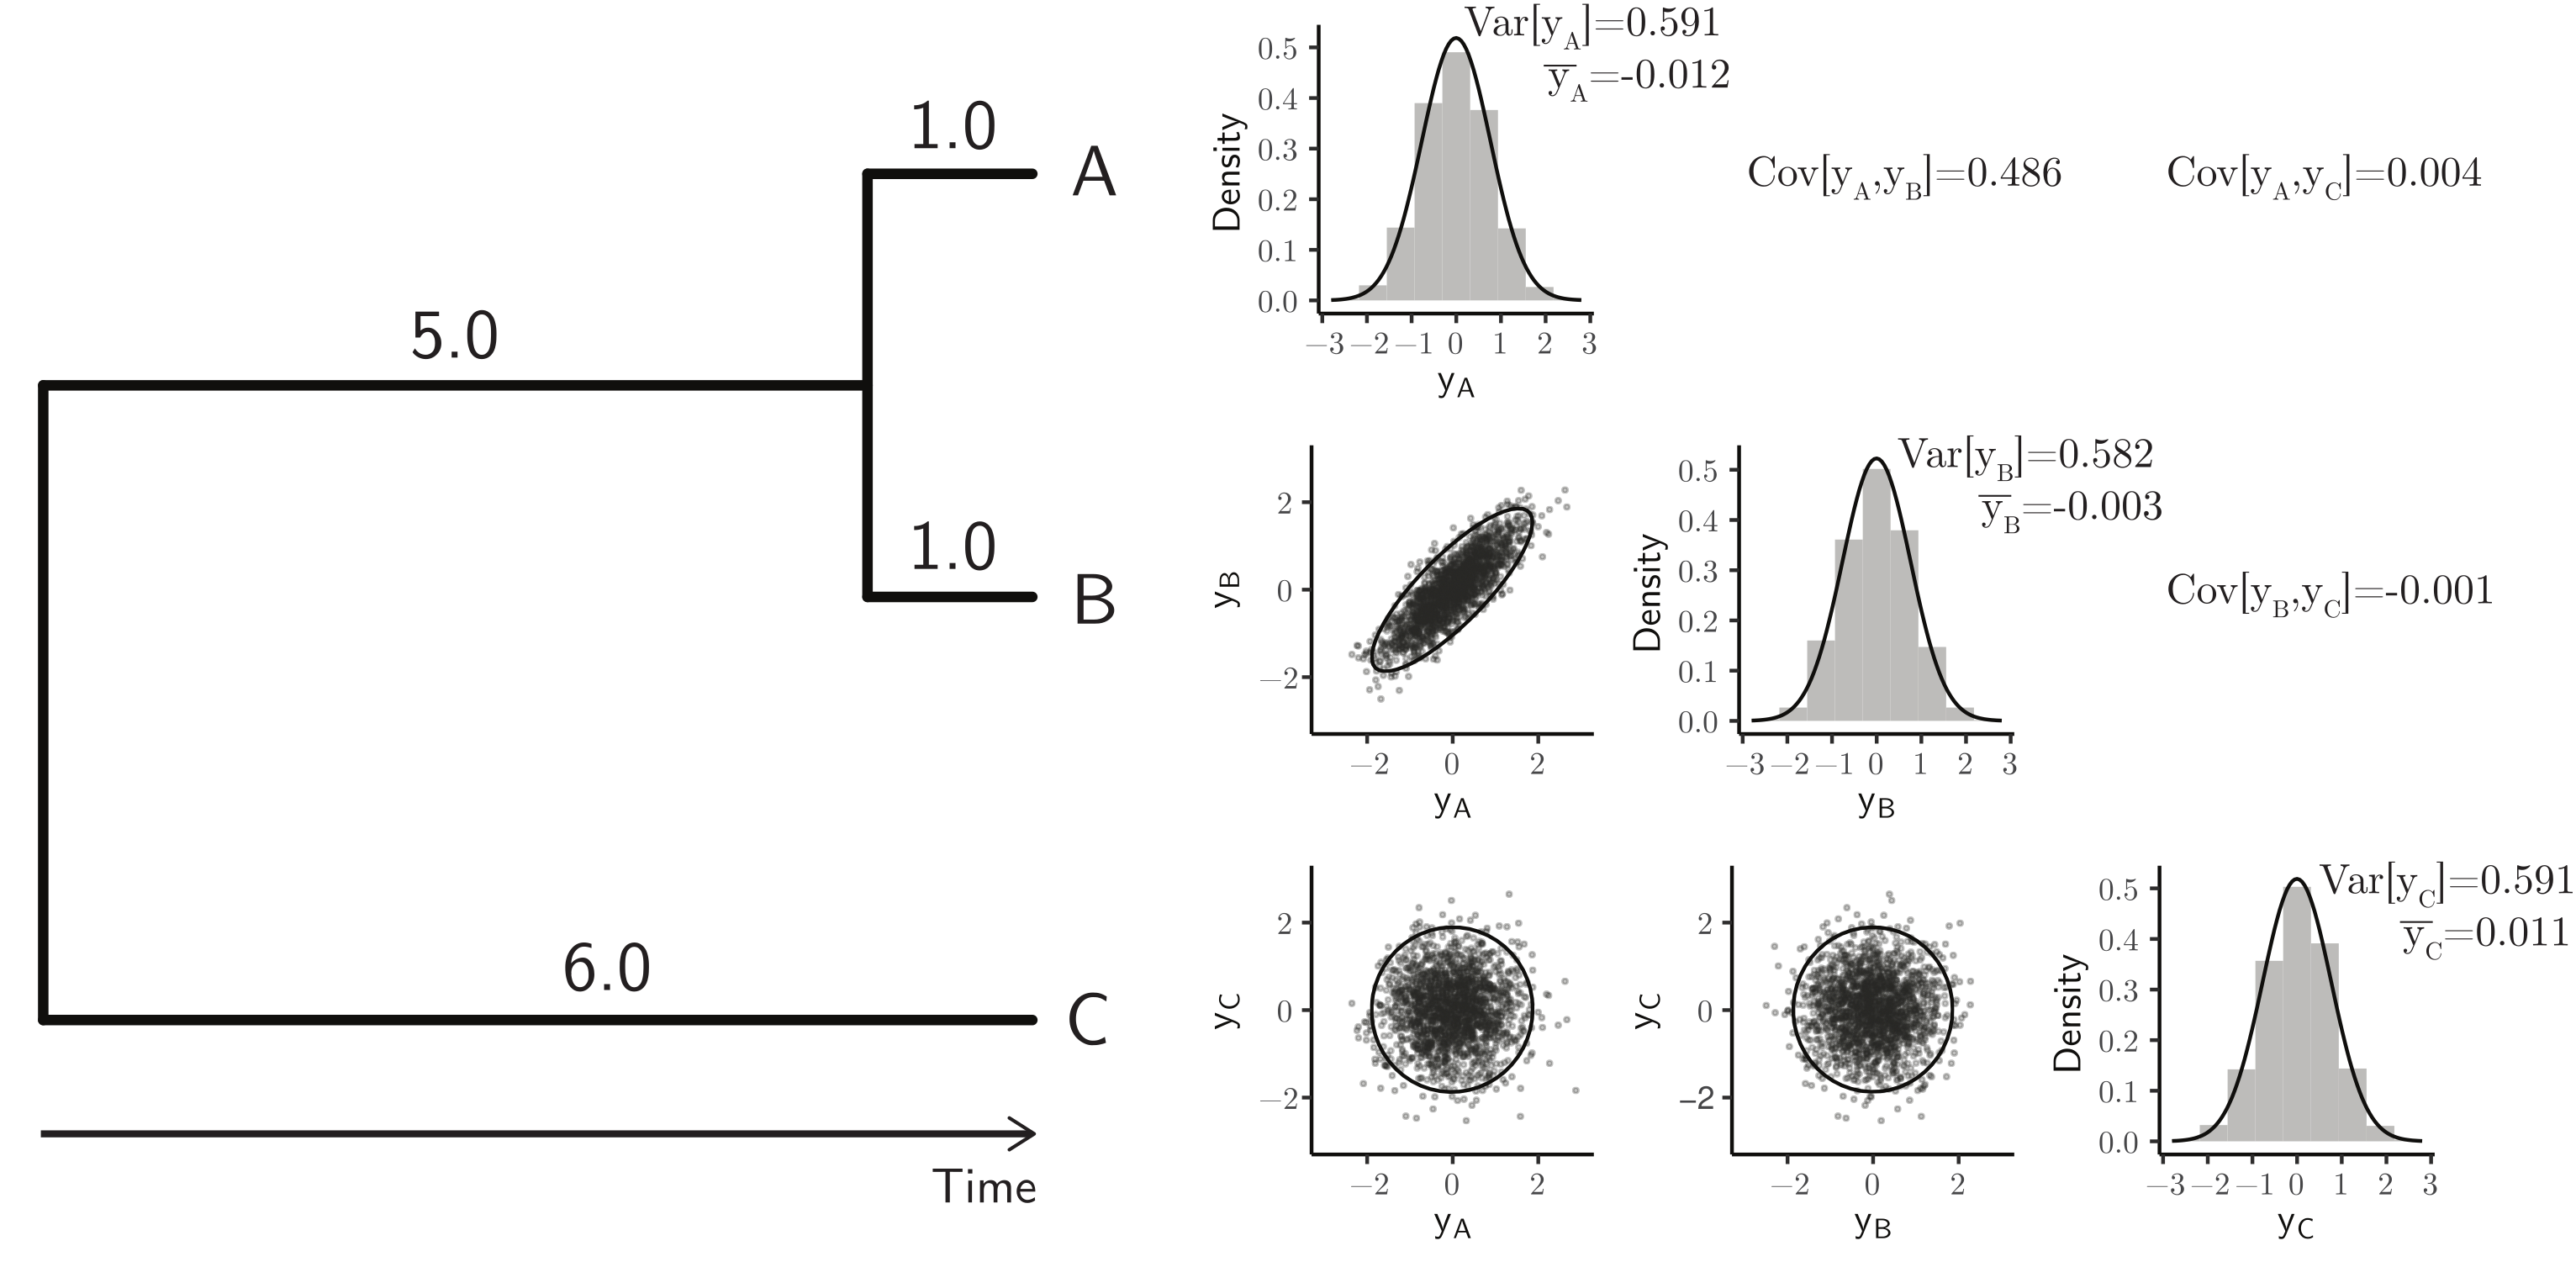
\includegraphics[width=11cm]{../figures/bmsim.pdf}
\label{fig:bmsim}
\DIFdelbegin %DIFDELCMD < \captionof{figure}{A sample of 200 draws from a MVN distribution, each
%DIFDELCMD <   representing the evolutionary trajectory of one continuous trait along
%DIFDELCMD <   the species tree on the left. The root trait value, $\boldsymbol{y_0}$, and the
%DIFDELCMD <   evolutionary rate of the process, $r$, were set to 0.0 and 0.1, respectively. The panel on the right shows
%DIFDELCMD <   histograms of trait values sampled from the MVN for each species, as
%DIFDELCMD < well as their covariation.}
%DIFDELCMD < %%%
\DIFdelend \DIFaddbegin \captionof{figure}{
  A sample of 1000 draws from a MVN distribution, each
  representing the evolutionary trajectory of one continuous trait along
  the species tree on the left. The root trait value, $\boldsymbol{y_0}$, and the
  evolutionary rate of the process, $r$, were set to 0.0 and 0.1, respectively.
  The panel on the right shows histograms of 1000 trait values sampled
  from the MVN for each species, as well as their covariation.}
\DIFaddend \end{center}

\DIFdelbegin %DIFDELCMD < \vspace{.25cm}
%DIFDELCMD < %%%
\DIFdelend %DIF >  \vspace{.25cm}
\emph{Validating a phylogenetic BM simulator}

\DIFdelbegin \DIFdel{Because the }\DIFdelend \DIFaddbegin \DIFadd{The }\DIFaddend MVN is a \DIFdelbegin \textbf{\DIFdel{known parametric
  distribution}}%DIFAUXCMD
\DIFdel{, it is trivial to verify the correctness of a
phylogenetic BM
model simulator, $S[f(\boldsymbol{y}|\boldsymbol{y_0},r,\boldsymbol{T})]$.
Figure }\DIFdelend \DIFaddbegin \DIFadd{well-characterized parametric distribution.
When used as the sampling distribution of the phylogenetic BM
process, it explicitly defines the expected trait value for
each species ($\boldsymbol{y_0}$), as well as their trait value
variances and covariances.
The latter comes from the variance-covariance matrix; for the
tree shown in figure }\DIFaddend 1 \DIFdelbegin \DIFdel{shows the result of 2000 simulations under the
MVN
with $\boldsymbol{y_0} = [0.0, 0.0, 0.0]$, }\DIFdelend %DIF >  \ref{fig:bmsim}
\DIFaddbegin \DIFadd{and with }\DIFaddend $r = 0.1$, \DIFdelbegin \DIFdel{along the tree shown on
the left, which determines the variance-covariance matrix
:
}\DIFdelend \DIFaddbegin \DIFadd{this matrix
is:
%DIF >  For example, given $\boldsymbol{y_0} = [0.0, 0.0, 0.0]$, $r = 0.1$, and $\boldsymbol{T}$
%DIF >  derived from the tree shown in figure \ref{fig:bmsim}
%DIF >  Because the MVN is a known parametric distribution, it is trivial to verify the correctness of a
%DIF >  phylogenetic BM model simulator, $\text{S}[f(\mathbf{y}|\boldsymbol{y_0},r,\boldsymbol{T})]$.
%DIF >  Figure 1 shows the result of 200 simulations under the MVN
%DIF >  with $\boldsymbol{y_0} = [0.0, 0.0, 0.0]$, $r = 0.1$, along the tree shown on
%DIF >  the left, which determines the variance-covariance matrix:
}\DIFaddend \begin{equation}
  r\boldsymbol{T} = 0.1
  \begin{bmatrix}
    6 & 5 & 0\\
    5 & 6 & 0\\
    0 & 0 & 6
  \end{bmatrix}
  \label{eq:mat}
\end{equation}

\DIFdelbegin \DIFdel{One can then verify that the simulated mean trait values and their
variances in each species }\DIFdelend \DIFaddbegin \DIFadd{Together, variance-covariance matrix $r\boldsymbol{T}$ and
$\boldsymbol{y_0} = [0.0, 0.0, 0.0]$ characterize a
population of phylogenetically related species trait values
whose means are 0.0, variances are 6.0, and co-variances
are 5.0 (between species ``A'' and ``B'') and 0.0 (between
species ``C''and
either ``A'' or ``B'').
}

\vspace{.25cm}

\DIFadd{Figure 1 shows the distributions of trait values and their variances
and covariances for one sample of \textcolor{red}{X} independent
realizations of phylogenetic BM processes.
One can see that the sample's average trait value and the
variances and covariances approach their expectations.
In order to be igorous, one can follow the method described
in the main text and verify that those expectations }\DIFaddend fall within
their 95\% confidence intervals 95\% of the time\DIFdelbegin \DIFdel{.
More specifically (i) $\boldsymbol{y_{\text{A}}}$, $\boldsymbol{y_{\text{B}}}$ and 
$\boldsymbol{y_{\text{C}}}$ fall within $[]$ X, Y and Z times out of 200, and 
(ii) $\text{Var}[\boldsymbol{y_{\text{A}}}]$}\DIFdelend , \DIFdelbegin \DIFdel{$\text{Var}[\boldsymbol{y_{\text{B}}}]$ and
$\text{Var}[\boldsymbol{y_{\text{C}}}]$ 
fall within $[]$ X, Y and Z times out of 2000.
}\DIFdelend \DIFaddbegin \DIFadd{as calculated
from a large number of samples (Supplementary Fig. \ref{supfig:bmsimcis} and
Supplementary Table \ref{suptab:bmsimcis}).
}\DIFaddend %
%\vspace{.25cm}
%\emph{Validating a phylogenetic BM likelihood implementation}
%
% For a small tree, the likelihood of a set
% of parameter values $\theta$ given some observed data is
% straightforward to compute (following Eq. \ref{eq:bm}) and can be compared to
% the output of a focal implementation.
% Interestingly, the likelihood of the BM model can also be computed using a
% dynamic-programming algorithm known in the phylogenetics literature
% as the ``pruning'' or ``peeling'' algorithm \citep{felsenstein73}.
% Thus, if a BM model is implemented correctly, the resulting likelihood
% of $\theta$ should match the solution of equation 2 no matter
% which algorithm is used.
\end{tcolorbox}
% End: BM BOX

\DIFdelbegin \DIFdel{Another example is the Yule model (also known as the pure-birth model;
\mbox{%DIFAUXCMD
\citealt{yule24}}\hspace{0pt}%DIFAUXCMD
), a continuous-time Markov process that has been
classically employed in phylogenetics to model the number of
species in a clade \mbox{%DIFAUXCMD
\citep{yule24,aldous01}}\hspace{0pt}%DIFAUXCMD
.
Under a Yule process with a species birth rate of $\lambda$, the
expected tree height, $\text{E}[t_{\text{root}}]$, for
a tree with $n$ tips is:
}%DIFDELCMD < 

%DIFDELCMD < %%%
\DIFdelend \begin{equation}
  \text{E}[t_{\text{root}}] = \sum_{i=2}^{n}\frac{1}{1\lambda}.
  \label{eq:yule}
\end{equation}

\noindent One can then verify if $\text{E}[t_{\text{root}}]$ is $95\%$
of the time within $\pm 1.96$ standard errors of the average
\DIFdelbegin \DIFdel{Yule-simulated tree
height }\DIFdelend \DIFaddbegin \DIFadd{Yule-tree height (from each sampled data set)}\DIFaddend .
Confirming that this is the case indicates \DIFdelbegin \DIFdel{$S[f(\Phi|\lambda)]$ }\DIFdelend \DIFaddbegin \DIFadd{$\text{S}[f(\Phi|\lambda)]$ }\DIFaddend is correctly
implemented (Fig. \ref{fig:yulemean}).
\DIFaddbegin \DIFadd{In Box 1, we illustrate this procedure for the (parametric) sampling distribution
underlying the phylogenetic Brownian motion model (``PhyloBM''; \mbox{%DIFAUXCMD
\citealp{felsenstein73}}\hspace{0pt}%DIFAUXCMD
).
Protocols for validating $\text{I}[\mathcal{M}]$ (see below) will also automatically validate
$\text{S}[\mathcal{M}]$.
}\DIFaddend 

\begin{figure}
  \centering
  \vspace{0pt}
  \begin{subfigure}[t]{0.5\textwidth}
    \caption{}
    \centering
    \begin{tabular}{ c|c }
    \hline
    Birth rate ($\lambda$) & E[$t_{\text{root}}$] $\in$ 95\% CI (\%)\\
    \hline  
    0.5 & 94\\
    0.6 & 91\\
    0.7 & 98\\
    0.8 & 95\\
    0.9 & 96\\
    1.0 & 92\\
    \hline
  \end{tabular}
  \end{subfigure}
  \vspace{0pt}
  \hspace{1cm}
  \begin{subfigure}[t]{0.4\textwidth}
    \caption{}
    \centering
    \DIFdelbeginFL %DIFDELCMD < \includestandalone[width=7cm]{../r_scripts/yule_exp_height}    
%DIFDELCMD <   %%%
\DIFdelendFL \DIFaddbeginFL \includestandalone[width=7cm]{../figures/yule_exp_height}    
  \DIFaddendFL \end{subfigure}
  \hfill
  %DIF > LM TODO: think about uncertainty intervals for coverage.
  \caption{Validation of Yule tree simulator.
    (a) Number of simulated data sets (out of 100) for which the
    expected tree height ($t_{\text{root}}$) was inside the 95\% CI
    about its sample average.
    Each data set consisted of 50 twenty-taxon simulated Yule trees.
    (b) The area shaded in light blue represents the
    95\% confidence interval about the average tree height, obtained
    from the 5,000 Yule trees simulated in (a). Simulations were
    carried out with the \texttt{TreeSim} R package \citep{stadler11}.}
  \label{fig:yulemean}
\end{figure}

We note that \DIFdelbegin \DIFdel{$S[\mathcal{M}]$ represents }\DIFdelend \DIFaddbegin \DIFadd{we have so far used $\text{S}[\mathcal{M}]$ to represent }\DIFaddend a \emph{direct} simulator
under model $\mathcal{M}$ (Table \ref{tab:sim}), meaning each and every sample
generated by \DIFdelbegin \DIFdel{$S[\mathcal{M}]$ }\DIFdelend \DIFaddbegin \DIFadd{$\text{S}[\mathcal{M}]$ }\DIFaddend is
independent.
This is contrast with other simulation strategies, such as conducting
MCMC under model $\mathcal{M}$ with no data, given specific parameter
($\boldsymbol{\theta}$) values.
This latter approach may be the only option if \DIFdelbegin \DIFdel{$S[\mathcal{M}]$ }\DIFdelend \DIFaddbegin \DIFadd{$\text{S}[\mathcal{M}]$ }\DIFaddend has not
been yet implemented, and it is predicated upon the existence of correct
implementations of both an inferential engine \DIFdelbegin \DIFdel{$I[\mathcal{M}]'$ }\DIFdelend \DIFaddbegin \DIFadd{$\text{I}[\mathcal{M}]'$ }\DIFaddend and of
proposal functions.
We distinguish \DIFdelbegin \DIFdel{$I[\mathcal{M}]'$ from $I[\mathcal{M}]$ }\DIFdelend \DIFaddbegin \DIFadd{$\text{I}[\mathcal{M}]'$ from $\text{I}[\mathcal{M}]$ }\DIFaddend because
simulations are being carried out precisely to validate \DIFdelbegin \DIFdel{$I[\mathcal{M}]$}\DIFdelend \DIFaddbegin \DIFadd{$\text{I}[\mathcal{M}]$}\DIFaddend .
Unless MCMC simulations are done with \DIFdelbegin \DIFdel{$I[\mathcal{M}]'$ }\DIFdelend \DIFaddbegin \DIFadd{$\text{I}[\mathcal{M}]'$ }\DIFaddend -- an independent
implementation of \DIFdelbegin \DIFdel{$I[\mathcal{M}]$ }\DIFdelend \DIFaddbegin \DIFadd{$\text{I}[\mathcal{M}]$ }\DIFaddend -- they can introduce circularity 
to the validation task.

\begin{center}
  \DIFdelbegin %DIFDELCMD < \begin{table}
%DIFDELCMD <   %%%
\DIFdelendFL \DIFaddbeginFL \begin{table}[h]
  \DIFaddendFL \caption{A non-exhaustive list of direct simulation software commonly used in evolutionary
    biology analyses.}
  \label{tab:sim}
  \centering
  \begin{tabular}{ p{0.7in} | p{1.3in} | p{1in} | p{1.1in} }
    \hline
    Software package & Model type & Platform & Reference \\
    \hline  
    Seq-Gen & Molecular sequence evolution models & Standalone & \citealp{rambaut97} \\
    ms & Coalescent model & Standalone & \citealp{hudson02}\\
    SLiM & Population genetic models & Standalone & \citealp{haller19}\\
    TreeSim & Birth-death models & R & \citealp{stadler11}\\
    mvMORPH & Continuous trait evolution models & R &
                                                      \citealp{clavel15}\\
    phytools & Several phylogenetic models & R & \citealp{revell12}\\
    MASTER & Continuous-time Markov (tree) models & BEAST 2 & \citealp{vaughan13}\\
    \hline
  \end{tabular}
  \end{table}
\end{center}

% If we determine $S(M)$ samples $\text{P}_{\text{S}}(\theta)$ directly (i.e.,
% there is no data $D$; ``S'' for \textbf{s}imulation), then $I(M)$
% samples $\text{P}_{\text{I}}(\theta)$ (``I'' for \textbf{i}nference),
% and we ultimately want $\text{P}_{\text{I}}(\theta)$ to reach
% stationarity at $\text{P}_{\text{S}}(\theta$) (see box 2). 

% \begin{tcolorbox}[breakable, width=12cm, colback=gray!10, boxrule=0pt,
%   break at=11cm/0cm, title=Box 1: Models with well-known parametric \emph{pdf}'s, fonttitle=\bfseries]

% To verify correctness of a simulator implementation \(S\) for model
% \(M\) directly, the distributions \(p_S(\theta|M)\) should match
% expected distribution based on theory. We can verify this by drawing a
% large number of samples using \(S\), calculate summary statistics on the
% sample and compare these with analytical estimates for these statistics.
% For example, for tree priors, expected tree heights can often be determined, and for parametric distributions we often know mean and variance values. Simulating values and making sure the expected value is in the expected range is easy to verify in Tracer: the expected values should be within the mean value logged plus/minus 2 times stderr of mean (as shown in the summary statistics panel).

% When no analytical estimates of statistics are available, it may be possible to find a simplified case (e.g. by leaving out any trees) which can be done analytically.

% Some examples of direct simulators (this list is far from exhaustive):

% \begin{itemize}
% \item
%   the \href{http://tgvaughan.github.io/MASTER/}{MASTER} (\cite{vaughan2013stochastic}) 
%   BEAST 2 package is a general purpose package for
%   simulating stochastic population dynamics models which can be
%   expressed in terms of a chemical master equation.
% \item
%   SimSnap for SNAPP (\cite{bryant2012inferring}) is a custom build
%   implementation in C++ for simulating alignments for a fixed tree and
%   SNAPP parameters.
% \item
%   The \texttt{beast.app.seqgen.SequenceSimulator} class in BEAST 2 can
%   be used to simulate alignments for general site models using
%   reversible substitution models. See
%   \href{https://github.com/CompEvol/beast2/blob/master/examples/testSeqGen.xml}{testSeqGen.xml}
%   for an example.
% \item
%   Models implemented in other phylogenetic software packages, such a
%   BEAS 1, MrBayes, RevBayes, allow sampling a distribution using MCMC.
% \item
%   The \texttt{beast.core.DirectSimulator} class in BEAST 2 can be used
%   to draw samples from distributions in BEAST that extend
%   \texttt{beast.core.distribution.Distribution} and implement the
%   \texttt{sample(state,\ random)} method. You can set up an XML file and
%   run it in BEAST. Here are a few examples:
%   \href{https://github.com/CompEvol/beast2/blob/master/examples/testDirectSimulator.xml}{testDirectSimulator.xml},
%   \href{https://github.com/CompEvol/beast2/blob/master/examples/testDirectSimulator2.xml}{testDirectSimulator2.xml},
%   and
%   \href{https://github.com/CompEvol/beast2/blob/master/examples/testDirectSimulatorHierarchical.xml}{testDirectSimulatorHierarchical.xml}.
% \end{itemize}

\subsubsection*{Validating the inferential engine, \DIFdelbegin \DIFdel{$I(M)$}\DIFdelend \DIFaddbegin \DIFadd{$\text{I}[\mathcal{M}]$}\DIFaddend }
\DIFaddbegin \label{sec:sbc}
\DIFaddend 

\DIFaddbegin \DIFadd{The more complex the natural phenomenon under study,
the more difficult it will be to strike a good balance
between model practicality and realism.
}\begin{wrapfigure}{l}{6.85cm}
  \label{fig:flowchart}
  %DIF >  \includestandalone[width=6.75cm]{../figures/flowchart}
  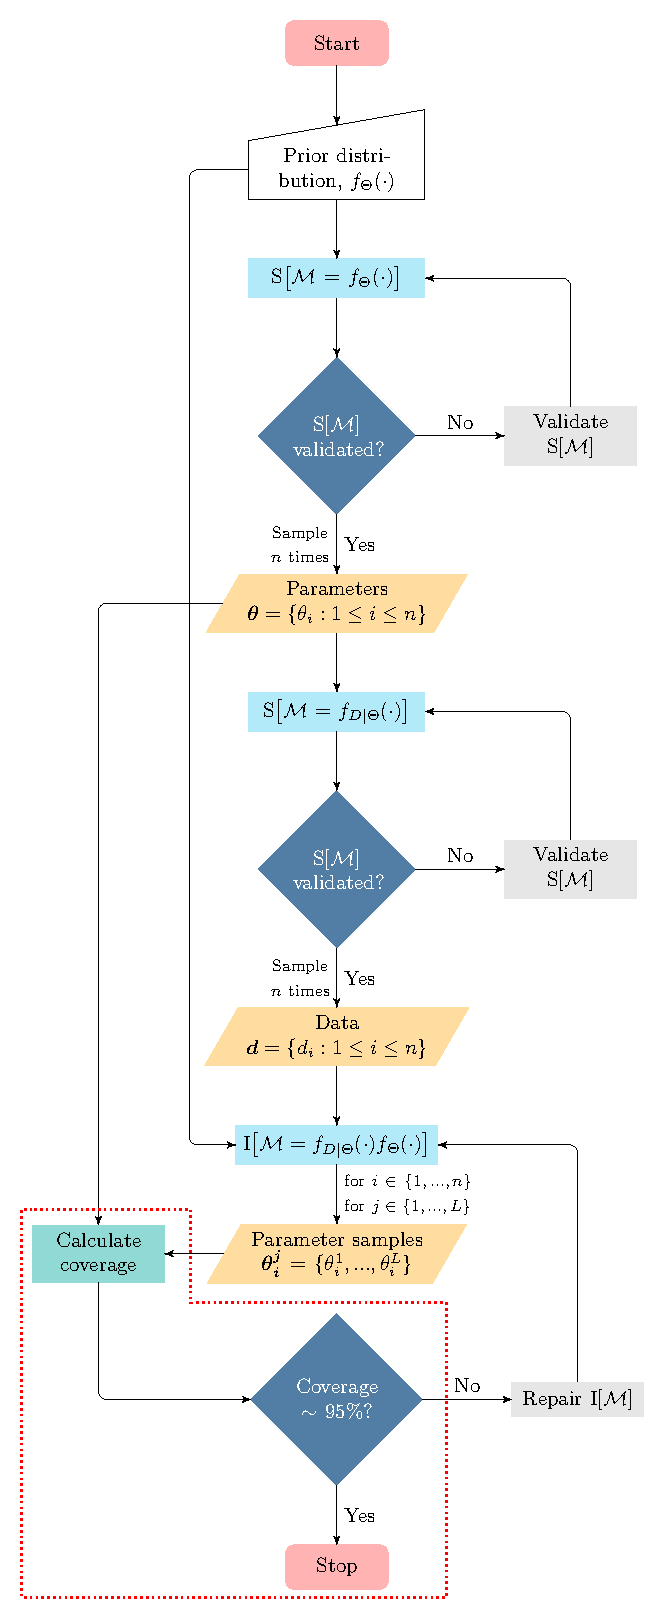
\includegraphics[width=6.75cm]{../figures/flowchart.pdf}
  \caption{\DIFadd{The several steps involved in determining a Bayesian model is
    well-calibrated. Note that even though we present simulation in two
    , one for prior $f_\Theta(\cdot)$ and one for the likelihood
    $f_D(\cdot|\theta)$, a Bayesian model $\mathcal{M}$ is 
    defined by the density functions of both prior and likelihood.}}
\end{wrapfigure}
\DIFadd{The popular aphorism rings true: ``all models are wrong but some are useful''
\mbox{%DIFAUXCMD
\citep{box79}}\hspace{0pt}%DIFAUXCMD
.
Very simple models are easier to implement in efficient inference tools, but will
commonly make assumptions likely to be broken by the data (e.g.,
\mbox{%DIFAUXCMD
\citealp{sullivan97,mendes17,mendes19}}\hspace{0pt}%DIFAUXCMD
).
Conversely, complex models will fit the data better (e.g., \mbox{%DIFAUXCMD
\citealp{ogilvie22}}\hspace{0pt}%DIFAUXCMD
), but
may become unwieldly with increasing levels of realism.
}

\DIFadd{A large number of parameters can cause overfitting and unidentifiability,
and highly complex models might lead to prohibitively slow inferential analyses
(e.g., \mbox{%DIFAUXCMD
\citealp{lartillot11}}\hspace{0pt}%DIFAUXCMD
).
%DIF >  In order to achieve correct inferences, it is of utmost importance to guarantee that inferential machinery returns quantifiably correct answers.
%DIF >  In practice, however, this is impossible to achieve due to the models under consideration being almost always badly misspecified for the data at hand.
Deciding on the utility of a model for real-world problems is a
daunting task \mbox{%DIFAUXCMD
\citep{brown18,shepherd18}}\hspace{0pt}%DIFAUXCMD
, and is a challenge we do not address in
the present contribution.
Such model appraisals are normally carried out after a model is
published, often in multiple contribution bouts, and are critical for a model's
longevity.
Analyses of model fit against data are normally accompanied by discussions on
assumption validity, and more rarely by benchmarking and scrutinization of model
behavior and implementation (e.g., \mbox{%DIFAUXCMD
\citealp{maddison07,rabosky15,rabosky13,moore16,stadler10,luo20}}\hspace{0pt}%DIFAUXCMD
).
}

\DIFadd{When a new model $\mathcal{M}$ is initially proposed, however, authors must ensure
that their methods
%DIF >  Simulating data from a probabilistic generative model can thus be helpful to understand when the inferential machinery under development
can at the very least robustly recover generating parameters.
In this section, we discuss a few techniques that can be employed to assess
the correctness of a parameter-estimation routine.
These techniques assume that one can simulate from a probabilistic data-generating
process (see previous section).
}

\vspace{.25cm}

\noindent{\emph{Coverage-validation of a Bayesian model \textcolor{red}{[@Luiz: or some other header if there is better terminology for this]}}}

\DIFadd{Our discussion on how to ensure a Bayesian model is well-calibrated
and thus correct will mostly follow the ideas in \mbox{%DIFAUXCMD
\citet{Cook2006} }\hspace{0pt}%DIFAUXCMD
and \mbox{%DIFAUXCMD
\citet{Talts2018}}\hspace{0pt}%DIFAUXCMD
.
The basic idea is presented in the flowchart in figure \ref{fig:flowchart}, and
consists of three stages: simulation, inference, and coverage calculation.
Once we have a validated simulator for model $\mathcal{M}$, we start by sampling $n$ parameter
sets from }\st{$\theta^{(i)}, i = 1, \ldots, M$} \DIFadd{$\boldsymbol{\theta} = \{\theta_1,\theta_2,...,\theta_n\}$
from its prior, }\st{$\pi(\theta)$} \DIFadd{$f(\theta)$.
For each parameter set $\theta_i$, we then sample a data set }\st{$y^{(i)}$} \DIFadd{$d_i$ from
}\st{$f(y^{(i)} \mid \theta^{(i)})$} \DIFadd{$f(d|\theta)$.
These two steps conclude the ``simulation'' stage of this validation
protocol.
With $\boldsymbol{d} = \{d_1,d_2,...,d_n\}$, we use the inferential machinery $\text{I}[\mathcal{M}]$ under
evaluation to compute }\st{$p(\theta \mid y^{(i)})$} \DIFadd{$f(\theta|d)$ for each $d_i$.
Recall that we assume the posterior distribution defined by $f(\theta|d)$ over $\theta$
will be approximated with MCMC, an algorithm that generates a large sample of size $L$ of
parameter values given a data set ($d_i$), $\boldsymbol{\theta}_i^{j}=\{\theta_1^1,\theta_1^2,...,
\theta_1^L\}$ }\st{$\boldsymbol\theta_s^{(i)} = \{\theta_{s1}^{(i)}, \ldots, \theta_{sL}^{(i)}\}$ of size $L$}\DIFadd{.
At this point, we have concluded the inference stage of this validation pipeline.
}

%DIF >  \noindent \emph{Well-calibrated validation study}
%DIF >  \textcolor{red}{FKM will fill this section.}
\DIFadd{The third stage and final stage consists of investigating coverage properties
of uncertainty intervals.
The critical expectation here is that if the inferential engine is correct, we will be able
to obtain interval estimates with precise coverage properties.
More concretely, let us first define the highest posterior density (HPD) interval.
For a credibility level $\alpha \in (0, 1)$, we define $I_\alpha(y) := (a(y, \alpha), b(y, \alpha))$
such that
}

\begin{center}
  \DIFadd{\hspace{0cm}
  }\cancel{$\frac{1}{m(y)} \int_{a(y, \alpha)}^{b(y,\alpha)} f(y \mid t)\pi(t)\,dt = \alpha$,}
\end{center}

\begin{equation*}
  \DIFadd{\frac{1}{f(d)} \int_{a(y, \alpha)}^{b(y,\alpha)} f(d | \theta)f(\theta)\, d\theta = \alpha,
}\end{equation*}

\DIFaddend \noindent \DIFdelbegin \emph{\DIFdel{Well-calibrated validation study}}
%DIFAUXCMD
\DIFdelend \DIFaddbegin \DIFadd{where }\st{$m(y) = \int_{\Theta} f(y \mid t)\pi(t)\,dt$} \DIFadd{$f(d) = \int_\Theta f(d|\theta)f(\theta)d\theta$
is a constant that can be ignored.
By defining $\text{Cred}(I_\alpha(y)) = \alpha$,
}\DIFaddend 

\DIFdelbegin \DIFdel{\textcolor{red}{FKM will fill this section.}
}\DIFdelend \DIFaddbegin \begin{center}
  \DIFadd{\hspace{0cm}
  }\cancel{$\inf_{b(y, \alpha)-a(y, \alpha)} \left \{ I_\alpha(y) : \text{Cred}(I_\alpha(y)) = \alpha \right\}$}
\end{center}
\DIFaddend 

%DIF >  \begin{equation*}
\DIFaddbegin 

%DIF >  \end{equation*}

\noindent \DIFadd{yields the shortest interval with the required credibility.
%DIF >  We are now prepared to discuss how to validate a (Bayesian) inference engine.
%DIF >  Consider the following generative model:
Now taking a set of parameter values $\theta_1$, and data points $d_1$,
sampled from $f_\Theta(\cdot)$ and $f_D(\cdot|\theta)$, respectively:
}

\begin{align*}
 \DIFadd{\xout{\theta_0} \theta_1 }&\DIFadd{\sim \xout{\Pi} f_\Theta(\cdot),}\\
 \DIFadd{\xout{\tilde{y}} y_1 }& \DIFadd{\sim \xout{F(\cdot \mid \theta_0)} f_D(\cdot | \theta_1),
}\end{align*}

\noindent \DIFadd{it can be shown that }\sout{$\operatorname{Pr}\left(\theta_0 \in I_\alpha(Y) \right) = \alpha$}
\DIFadd{$\operatorname{Pr}\left(\theta_1 \in I_\alpha(d) \right) = \alpha$, i.e., that $100\times\alpha$\% HPDs
have nominal coverage under the true generative model.
A proof is provided in the supplementary material.
}

%DIF >  \begin{figure}
%DIF >    \label{fig:flowchart}
%DIF >    \includestandalone[width=8cm]{../figures/flowchart}
%DIF >  \end{figure}

\DIFaddend \begin{table}
\begin{center}
\DIFdelbeginFL %DIFDELCMD < \begin{tabular}{lc}
%DIFDELCMD < %%%
\DIFdelendFL \DIFaddbeginFL \begin{tabular}{l|c}
\DIFaddendFL \hline
\DIFdelbeginFL \DIFdelFL{k }\DIFdelendFL \DIFaddbeginFL \DIFaddFL{$k$ }\DIFaddendFL & \DIFdelbeginFL \DIFdelFL{$\text{P}(x=k)$ }\DIFdelendFL \DIFaddbeginFL \DIFaddFL{$\text{Pr}(x=k)$ }\DIFaddendFL \\ % & $\text{P}(x\le k)$ & $\text{P}(x\ge k)$\\
\hline
90 & 0.0167 \\ % & 0.0282 & 0.9718\\
91 & 0.0349 \\ % & 0.0631 & 0.9369\\
92 & 0.0649 \\ % & 0.1280 & 0.8720\\
93 & 0.1060 \\ % & 0.2340 & 0.7660\\
94 & 0.1500 \\ % & 0.3840 & 0.6160\\
95 & 0.1800 \\ % & 0.5640 & 0.4360\\
96 & 0.1781 \\ % & 0.7422 & 0.2578\\
97 & 0.1396 \\ % & 0.8817 & 0.1183\\
98 & 0.0812 \\ % & 0.9629 & 0.0371\\
99 & 0.0312 \\ % & 0.9941 & 0.0059\\
100 & 0.0059 \\ % & 1.0000 & 0.0000\\
\hline
\end{tabular}
\end{center}
\caption{Under a correctly implemented model, coverage \DIFaddbeginFL \DIFaddFL{$x$ }\DIFaddendFL (the number
  \DIFdelbeginFL \DIFdelFL{$k$
  }\DIFdelendFL of true simulated values that fall within their corresponding 95\%-HPDs)
  is binomially distributed \DIFdelbeginFL \DIFdelFL{, }\DIFdelendFL with \DIFaddbeginFL \DIFaddFL{$n$ trials ($n=100$ in this case),
  and probability of success }\DIFaddendFL $p=0.95$.\DIFdelbeginFL %DIFDELCMD < \label{tab:coverage}%%%
\DIFdelendFL }
\DIFaddbeginFL \label{tab:coverage}
\DIFaddendFL \end{table}

\begin{figure}
  \includegraphics[width=\textwidth]{../figures/yule_calval.pdf}
  \caption{\DIFdelbeginFL \DIFdelFL{Calibrated validation }\DIFdelendFL \DIFaddbeginFL \DIFaddFL{\textcolor{red}{[This figure is being updated]}
    Coverage-validation }\DIFaddendFL analyses of a simple Bayesian
    hierarchical model \DIFdelbeginFL \DIFdelFL{. }\DIFdelendFL (\DIFdelbeginFL \DIFdelFL{a}\DIFdelendFL \DIFaddbeginFL \DIFaddFL{Fig. \ref{fig:pgm}}\DIFaddendFL )\DIFdelbeginFL \DIFdelFL{The graphical representation of the model used in
    the analyses, where $\lambda$ is the Yule birth-rate, $n$ is the
    number of species, and $\tau$ is the set of speciation times}\DIFdelendFL . \DIFdelbeginFL \DIFdelFL{The
    prior is an exponential density with arbitrary mean of 0.01. }\DIFdelendFL Panels \DIFdelbeginFL \DIFdelFL{(b-d)
    }\DIFdelendFL show \DIFaddbeginFL \DIFaddFL{the }\DIFaddendFL true
    \DIFdelbeginFL \DIFdelFL{$\lambda$ }\DIFdelendFL \DIFaddbeginFL \DIFaddFL{(i.e., simulated or generating) parameter }\DIFaddendFL values plotted
    against their mean posteriors (the dashed line gives $f(x) = x$).
    \DIFdelbeginFL \DIFdelFL{(b) Trees
    with $50<n<200$}\DIFdelendFL \DIFaddbeginFL \DIFaddFL{Dots and lines represent true values and their 95\%-HPDs}\DIFaddendFL ,
    \DIFaddbeginFL \DIFaddFL{respectively.
    Simulations for which 95\%-HPDs contained the true value are
    highlighted in blue, otherwise are presented in red.
    }\DIFaddendFL (\DIFdelbeginFL \DIFdelFL{c}\DIFdelendFL \DIFaddbeginFL \DIFaddFL{a}\DIFaddendFL ) \DIFdelbeginFL \DIFdelFL{Trees with $5<n<10$, }\DIFdelendFL \DIFaddbeginFL \DIFaddFL{Model is correctly specified. }\DIFaddendFL (\DIFdelbeginFL \DIFdelFL{d}\DIFdelendFL \DIFaddbeginFL \DIFaddFL{b}\DIFaddendFL ) Model is misspecified
    \DIFaddbeginFL \DIFaddFL{in inference }\DIFaddendFL (log-normal \DIFdelbeginFL \DIFdelFL{prior }\DIFdelendFL \DIFaddbeginFL \DIFaddFL{on $\lambda$ }\DIFaddendFL is \DIFdelbeginFL \DIFdelFL{used in inference}\DIFdelendFL \DIFaddbeginFL \DIFaddFL{misspecified).
    (c) Model is correctly specified}\DIFaddendFL , \DIFdelbeginFL \DIFdelFL{rather than exponential}\DIFdelendFL \DIFaddbeginFL \DIFaddFL{but only small trees (with
    up to fifteen taxa}\DIFaddendFL ) \DIFaddbeginFL \DIFaddFL{are generated}\DIFaddendFL .
  }
  \label{fig:yulecalval}
\end{figure}

\DIFaddbegin \DIFadd{The inference engine $\text{I}[\mathcal{M}]$ of a Bayesian model
is said to be well-calibrated and correct if we ascertain that the
coverage it produces lies within the expected bounds.
More specifically, the coverage of $n$ intervals obtained as above
will be distributed as binomial random variable with $n$ trials and
success probability $\alpha$.
When $n=100$ and $\alpha = 0.95$, the confidence interval for the
number of simulations containing the correct data-generating parameter
is between $90$ and $99$ (Table \ref{tab:coverage}).
}

\DIFadd{We provide an example in figure \ref{fig:yulecalval}, which shows 
coverage graphical summaries for the model represented in
figure \ref{fig:pgm}.
This model is deliberately simple for the sake of brevity and clarity
in the discussion below.
The parameters in this model are the phylogenetic tree $\Phi$, the
species birth rate $\lambda$, and the continuous-trait evolutionary rate
$r$ (we assume the continuous trait-root value, $\boldsymbol{y_0}$, is
known and set it to $\boldsymbol{0.0}$ for all simulated data sets).
When the model is correctly specified (Fig. \ref{fig:yulecalval}a),
coverage is close to 95\% and is adequate.
In figure \ref{fig:yulecalval}b, however, we misspecify the model
during inference, setting the prior distribution on
$\lambda$ to be a log-normal with  a mean of -2.25 (rather than -3.25,
as specified in the simulation procedure; Fig. \ref{fig:pgm}).
As can be seen, coverage is much lower (\textcolor{red}{X\%}), which
suggests that the model is not behaving as expected.
Of course, in a real-world validation experiment the model should
be correctly specified, and such a result would suggest a problem
with the inferential machinery (provided the the simulator has been
previously validated).
}

\DIFadd{Finally, we can further capitalize on this validation setup and
gauge how accurate our inferential tool can be for different
parameters. 
The more identifiable a parameter is, the higher should the
correlation between its posterior mean and its generating ``true''
value be.
In our first example (Fig. \ref{fig:yulecalval}a), the species
birth-rate $\lambda$ is largely identifiable for trees of the
simulated size (Fig. \ref{fig:yulecalval}a).
In a separate analysis, we analyzed the same model save for one
difference: phylogenetic trees could only have up to fifteen
terminal taxa.
The results are shown in figure \ref{fig:yulecalval}c.
Here, it can be seen that the inference machinery is less accurate
and that the $\lambda$ parameter is less identifiable.
We note that unidentifiability should not be taken as a sign that
a model is incorrect -- in figure \ref{fig:yulecalval}c, coverage
is still appropriate.
}

\vspace{.25cm}

\DIFaddend \noindent \emph{Simulation-based \DIFdelbegin \DIFdel{validation study}\DIFdelend \DIFaddbegin \DIFadd{calibration (SBC) \textcolor{red}{[@Luiz: Or any other
    header that makes sense, to help organize the inference validation section]}}\DIFaddend }

\DIFaddbegin \DIFadd{\mbox{%DIFAUXCMD
\cite{Talts2018} }\hspace{0pt}%DIFAUXCMD
show that one can devise other tests that might be
more powerful to detect problems than just looking at the coverage of
Bayesian HPD intervals.
In particular, they show (Theorem 1 therein) that if the inference machinery
$\text{I}[\mathcal{M}]$ works as intended, the distribution of the rank
}\st{$r^{(i)}$} \DIFadd{$r^j$ of the $j$-th sample from an MCMC chain ($\boldsymbol{\theta}^j
= \{\theta^1, \theta^2, ..., \theta^L\}$) }\st{in $\boldsymbol\theta_s^{(i)}$}
\DIFadd{will follow a uniform distribution on $[1, L + 1]$.
In other words, if one were to sort all $L$ samples from the output
of an MCMC experiment by a given parameter value, the first (smallest)
10\% of all samples should account for approximately 10\% of the total
posterior density; the next 10\% of (larger) samples should account, again,
for approximately 10\% of the total posterior density, and so on.
}\DIFaddend \textcolor{red}{\DIFdelbegin \DIFdel{FKM will run a SBV on a simple hierarchical model
  here}\DIFdelend \DIFaddbegin [\DIFadd{@Luiz: this was my shot at verbalizing the mathematical
  description}\DIFaddend . \DIFaddbegin \DIFadd{Is this correct?}]\DIFaddend }
\DIFaddbegin \DIFadd{Adherence to this distribution can be investigated by constructing
histograms \mbox{%DIFAUXCMD
\citep{Talts2018} }\hspace{0pt}%DIFAUXCMD
as well as by looking at the empirical
cumulative distribution function (ECDF) and their confidence bands
\mbox{%DIFAUXCMD
\citep{Sailynoja2021}}\hspace{0pt}%DIFAUXCMD
.
}\DIFaddend 

\DIFaddbegin \DIFadd{We illustrate the SBC procedure on the model represented in figure
\ref{fig:pgm}... \textcolor{red}{[@Remco or @Luiz: to be done]}
}

\DIFadd{\textcolor{red}{
  Items to discuss/consider after example:
  \begin{itemize}
  \item Would it help to have a flowchart for the SBC procedure?
  \item What happens when the distribution of ranks is not uniform,
    and is, say, shifted towards low or high ranks? How can this help
    us fix or understand a model better? (see second point below);
  \item Show how a misspecified model can cause this test to fail
    (if we take the Yule + phyloBM model as an example, as I suggest,
    there are only a few parameters to be misspecified, so maybe it's
    easy to get this test to fail and know exactly why. One way to do that
    with that model, I'd suspect, is to throw away all trees with
    fewer than, say, 15 leaves -- I would imagine that would distort
    our $\lambda$ rank distribution, even if the model still pass
    the well-calibrated test);
  \item What are the downsides of SBC relative to just verifying
    a model is well-calibrated? You'd have to simulate 1,000
    data sets instead of 100 (so you have, say, 100 per 10\% bin).
    Very computationally intensive!
  \item What are we going to recommend to the reader? That they
    really always go all the way to SBC? That's asking for too much.
    We have to argue that the first type of test is enough for
    correctness.
  \end{itemize}
}
}

\begin{tcolorbox}[breakable, width=\textwidth, colback=gray!10, boxrule=0pt,
  title=Box 1: Validating a phylogenetic model with respect to its
  phylogenetic tree parameter, fonttitle=\bfseries]
  \small 

  \DIFadd{Given the centrality of the phylogenetic tree ($\Phi$) in comparative
  analyses, we must pay close attention to how we investigate this
  parameter when validating a phylogenetic model.
  Analyzing phylogenetic trees is made challenging by tree space
  being a complex mix of a discrete and continuous component, due to
  trees being comprised by both a topology and set of node times
  \mbox{%DIFAUXCMD
\citep{semple03,gavryushkin16}}\hspace{0pt}%DIFAUXCMD
.
  Additionally, there is no canonical total-ordering  structure for
  trees, which complicates a validation procedure such as SBC.
}

  \vspace{.25cm}
  \DIFadd{To get around this difficulty, we propose computing one or more phylogenetic
  metrics, or functionals, for which total-ordering holds
  and thus for which ranks can be obtained.
  \textcolor{red}{[@Luiz: my suggestion is to focus on RF here]}
  One such metric is the well-known Robinson-Foulds distance (RF; \mbox{%DIFAUXCMD
\citealp{Robinson1981}}\hspace{0pt}%DIFAUXCMD
),
  which measures \textcolor{red}{[@Luiz: brief description of RF]}
  relative to another phylogenetic tree.
  In order to compute a relational metric like the RF distance during
  validation, we must have a reference phylogeny $\Phi_0$ to which
  we can compare our focal generating phylogeny $\Phi$ and its
  posterior MCMC samples.
  The simulation-based calibration protocol remains the same, with
  an additional step in which we generate $\Phi_0$ (see Algorithm
  \ref{alg:sbc} in the supplementary material).
  Figure \textcolor{red}{X [@Luiz: see my description of new Fig. X below]} shows
  validation results for the RF metric for trees simulated under the model
  illustrated in Fig \ref{fig:pgm}. 
  Figure \textcolor{red}{Xa} and \textcolor{red}{Xb} show the coverage of 95\%-HPD
  intervals, and the rank distribution of the RF metric, respectively.
  The coverage of the RF statistic is very close to 95, and the rank distribution
  is approximately uniform on (1,$L+1$); together, both panels indicate this model
  is correct.
  We consider other phylogenetic tree metrics that could be used as an alternative
  to RF in the supplementary material (Supplementary
  Figs. \ref{supfig:sbc} and \ref{supfig:phylo_calibration}).
}

  \DIFadd{\textcolor{red}{[@Luiz: include Fig Xa and FigXb here; this figure
    would consist of just the RF panels; all other metrics have would
    be placed in the supp. material]}
}\end{tcolorbox}

%DIF >  Note that a tree by itself does not allow one to simulate the observables (alignments). %TODO decide whether to include this
%DIF >  Obviously, one might choose to keep $\boldsymbol \alpha$ fixed during the procedure, but it this will not exactly assess the validity of the joint sampler. 
%DIF >  This is particularly important for phylogenetics because the relationship between phylogeny and other parameters non-linear.
%DIF >  One important general point about phylogenetic space is that it does not possess a canonical representation.
%DIF >  The BHV parametrisation is quite useful in that allows unique geodesics and admits central limit theorems, so maybe there is some theoretical justification for using BHV path lengths as the univariate representation -- i.e. the $\delta$ -- in phylo-SBC.

%DIF >  \paragraph{An example}

%DIF >  In order to illustrate how a typical phylogenetic SBC analysis might work, we discuss a simple example where [REMCO will describe this in detail].

  
\DIFaddend % There is a wide variation on the validation stringencies different
% methods and models are subjected to in the course of their
% development \citep{darriba18}.
% From a short literature review on Bayesian methods applied to
% phylogenetics (Table S1), we summarize {\color{red}{four [could be more
%     after literature review]}} main validation requirements,
% in increasing order of stringency and comprehensiveness,
% that model implementations can meet:

% \begin{enumerate}[i.]
%   \item the model produces reasonable estimates on a real data set,
%   \item the model likelihood evaluates to some theoretical
%     expectation and/or approximates an expected distribution,
%   \item the model often recovers the right parameter
%     values -- for one or more parameters (i.e., a small hand-picked
%     ``grid'' of values) -- from data sets simulated with $S(M)$, and
% \item the model correctly estimates parameter values from data sets
%   simulated from prior distributions, as indicated by the estimated
%   posterior coverage of parameters and their correlation with true
%   values (``well-calibrated validation'', see below). {\color{red}{If
%       we want to talk about the next level -- using other HPDs, we can
%       add it as the 5th possibility and expand on it below}}
% \end{enumerate}

% \vspace{.25cm}
% \noindent \emph{The model produces reasonable estimates on a real
%   data set}

% One initial yet insufficient step in validating a model implementation
% is verifying whether it produces reasonable inferences with a real
% data set.
% Depending on the particular biological question at hand, it is very
% hard or arguably impossible to know what the true, expected answer is,
% and so ``reasonable'' will always be up for debate.
% A reasonable inference could be one confirming a result from a previous study
% using the same data and model, or different data and model
% altogether, but contradictory inferences do not necessarily imply a model
% was incorrectly implemented.
% For this reason, this validation procedure cannot consist of a proper
% correctness check, but should instead be seen as an exploratory
% analysis or a sanity check (the latter would require massive
% evidence supporting a particular hypothesis).
% Accordingly, a large fraction of publications to date employ this
% strategy as a final step to illustrate the workings of a method more
% than to validate it (but see Table S1 in the supplementary material).

% \vspace{.5cm}
% \noindent \emph{The model likelihood evaluates to some
%   expected value or approximates an expected distribution}

% A good starting point in formally verifying the correctness of a
% probabilistic model implementation is the comparison between the
% likelihood of a parameter value given some data, $\text{P}(D|\theta)$, to
% some expected result.
% When models are sufficiently simple, or by focusing
% on a subcase of a complex model, it is often straightforward to derive
% what this expected result should be (see box 1).
% Using the Yule model again as an example, the probability of observing
% a phylogenetic tree $T$ given $n$ internal nodes and birth-rate
% $\lambda$ (i.e., the Yule's model likelihood function;
% \citealp{nee01}) is:

% \begin{equation}
%   \text{P}(T|n,\lambda) = (n-1)!\lambda^{n-2}e^{-\lambda L},
%   \label{eq:yulelik}
% \end{equation}

% \noindent where $L$ is the total length of the tree.
% Because likelihood functions are often computed in log-space, and
% because constants (e.g., the $(n-1)!$ term in Eq. \ref{eq:yulelik}) can be
% ignored during MCMC for efficiency, the log-likelihood function for the Yule model
% becomes:

% \begin{equation}
% \text{log P}(T|n,\lambda) = \text{log}(\lambda^{n-2}) - \lambda L.
% \end{equation}

% \noindent One can then easily compute the expected log-likelihood of an example
% tree given some $\lambda$ value by hand, and compare it against the
% value produced by the implementation being validated.
% This forms the basis of what software engineers refer to as ``unit
% testing'' (see the supplementary material for a unit test example
% under the BEAST 2 platform).
% Expected values can also be obtained from independent
% implementations of the likelihood function -- the more different the
% other implementation (e.g., different algorithms and programming
% languages are used), the more robust the test is (see box 1).

% \vspace{.25cm}
% \begin{tcolorbox}[breakable, width=\textwidth, colback=gray!10, boxrule=0pt,
%   title=Box 2: Additional validation sanity-checks, fonttitle=\bfseries]
%   \small

%   In addition to the validation procedures described in the main text,
%   method developers can opt to conduct sanity checks that will not
%   provide evidence for model correctness, but that can nonetheless
%   reveal something is wrong with the implementation of a likelihood
%   function (i.e., checks that are necessary but not sufficient).

%   \vspace{.25cm}
%   \emph{The score function}

%   One such check is looking at properties of the score function,
%   $U(\theta,D)=\frac{\partial}{\partial\theta}\log
%   \text{P}(D|\theta)$.
%   $U(\theta,D)$ is the gradient of the log-likelihood function with
%   respect to $\theta$ (the parameters in the model), thus indicating
%   the slope of $\text{P}(D|\theta)$ and its behavior given very small
%   changes in $\theta$.
%   Given a data set $D$ generated from one or more $\theta$ values, it
%   should be expected from a correct model implementation that:

%   \begin{equation}\label{eq:scorefunction}
%     \text{E}[U(\theta,D)] = \int U(\theta,D)\text{P}(D|\theta)dD = 0,
%   \end{equation}

%   This theoretical expectation can then be compared to the one
%   computed from a simulated data set (generated by $S(M)$; see the
%   supplementary material for more details).

%   \vspace{.25cm}
%   \emph{Comparing empirical vs. target posterior distributions}

%   Given a correctly implemented simulator for model $M$, $S(M)$, one
%   can directly generate a $\text{P}_{\text{S}}(\theta)$ distribution that
%   should be approximated by $\text{P}_{\text{I}}(\theta)$ at stationarity.
%   Note that under this validation scope, there is no data.
%   If chains are run long enough (as suggested by large effective
%   sample sizes, ESS's), $\text{P}_{\text{S}}(\theta)$ and
%   $\text{P}_{\text{I}}(\theta)$ can be compared, and large
%   discrepancies between them can be taken as evidence of an error in the
%   likelihood function implementation (assuming all other inferential
%   components are working properly).

%   \vspace{.15cm}
%   Such task can be done with a non-parametric test, for example, such
%   as the Kolgomorov-Smirnov test \citep{kolgomorov,smirnov,ks}, which
%   compares two empirical distribution functions (\emph{ecdf}'s) or an
%   \emph{ecdf} with a cumulative distribution function (\emph{cdf}).
%   We provide an example of this procedure in the supplementary material.
% \end{tcolorbox}

% Alternatively, a more comprehensive approach could involve comparing
% some expected quantity against its sampling distribution under the
% model being validated.
% This sampling distribution is often obtained through MCMC, with
% newly proposed parameter values being accepted in direct proportion to
% their likelihood under the model (i.e., this distribution comes from
% $I(M)$ without using any data, just a fixed $\theta$ value).
% Given a correct implementation of the Yule model,
% for example, the distribution of tree heights (for some $\lambda$
% value) should peak around the value given by from equation \ref{eq:yule}.
% This procedure is more comprehensive than unit testing because of its
% dependence on MCMC, which means a valid result requires correct
% implementations of both the likelihood function and the proposal mechanism.

% When analytical expectations are not available, the distribution
% sampled from $I(M)$ with MCMC, $\text{P}_{\text{I}}(\theta)$, can be
% compared to a target distribution sampled with $S(M)$
% ($\text{P}_{\text{S}}(\theta)$, see box 2).
% $S(M)$ can also be itself conveniently used by $I(M)$ as the proposal
% density during MCMC (see listing 2 in the supplementary material for
% an example).
% This allows isolating the validation task to the model:
% when other proposal densities are used, mismatched distributions can be
% due to malfunctioning of either or both model and proposal mechanism.

% \vspace{.5cm}
% \noindent \emph{The model often recovers the right parameter values
%   from data sets simulated at a (grid of) point(s) in parameter space}

% Perhaps the most common approach to date for validating a
% probabilistic model involves simulating data sets under specific parameter
% values -- the scope here requires a simulator $S(M)$ used to simulate
% \emph{data} under model $M$ -- carrying out inference, and tabulating
% estimates depending on how close they were to the known, true values.
% This procedure is particularly valuable in the context of point estimates
% that ignore uncertainty, characteristic of maximum-likelihood methods (e.g.,
% \citealp{mccormack09,han13,mendes17}), but of smaller if not unclear
% utility in the Bayesian framework.

% Differently from frequentist methods, which rely on approximate bootstrap
% analyses, Bayesian models allow for exact statistical inference while
% simultaneously addressing uncertainty.
% As a result, parameter estimates come in the form of a posterior
% distribution that depends not only on the model likelihood, but
% also the priors of choice.
% Validating a Bayesian model by trying to recover
% hand-picked parameter values can be problematic because it is unclear
% which prior is to be used, and also how often one should
% expect a specific highest posterior density (HPD) interval to contain
% the true parameter values.

% Presumably, correct model implementations should yield HPDs that contain
% the true values more often than not, but determining what ``often'' means
% for complex models and priors is not trivial.
% Thus, there are no theoretical guarantees that a model is correctly
% implemented should most inferred 95\% HPDs include the true parameter
% values, for example, or vice-versa.
%DIF >  LM: I thought so too, but it turns out that if you sample from the prior you *can* give guarantees.
% This validation approach can still be useful in revealing regions
% in parameter space where inference is easier or harder (given different
% prior distributions), but we instead recommend procedures that are exact,
% such as calibrated validation studies (see below).

% \vspace{.5cm}
% \noindent \emph{The model correctly estimates parameter values from
%   data sets simulated from prior distributions, as indicated by the
%   estimated posterior coverage}

% Rather than simulating a fixed number of data sets for hand-picked
% parameter values (see above), we can let the prior density of
% different values dictate how often they are used in simulations.
% This forms the basis of a calibrated validation study: a large number
% of data sets are simulated directly from the prior distributions on
% model parameters.
% Here, the choice of prior is arbitrary, but ideally should reflect
% what is currently known about the natural phenomenon being modeled.

% The advantage of this approach is that if the same Bayesian model (which
% includes likelihood \emph{and} priors) is used for both
% simulation and inference, there are clear expectations under a
% correctly implemented model.
% Namely, out of a large number of simulations, the coverage of a
% parameter should match the width of the HPD of choice
% (coverage is defined as the number of times the HPD
% interval contains the true value out of the total number of
% simulations; \citealp{dawid82}).
% For example, in the case of the commonly used 95\%-HPD interval, the true value
% should often be inside the HPD between 90--98\% of the time (Table
% \ref{tab:coverage}).


% Figure \ref{fig:yulecalval} shows the results of a calibrated
% validation analysis for a simple Bayesian model.
% Here, the full model is comprised of an exponential prior (with an
% arbitrary mean of 0.01) on the birth-rate
% $\lambda$, with the Yule likelihood (i.e., a pure-birth process)
% modelling speciation times $\tau$ (Fig. \ref{fig:yulecalval}a).
% We plot 100 ``true'' $\lambda$ values (drawn from the exponential prior)
% against their posterior means estimated through MCMC from the
% corresponding trees simulated under the Yule model
% (Fig. \ref{fig:yulecalval}b-d).
% Note that coverage is good for the first and second calibrated
% validation analyses (the vast majority of 95\%-HPDs
% include the true values, as shown by the blue vertical lines; Fig
% \ref{fig:yulecalval}b-c), for which the model was correctly
% specified.
% Coverage is not good in the third analysis, where the model was
% mispecified on purpose (a log-normal prior was used in inference,
% rather than an exponential; Fig. \ref{fig:yulecalval}d).
% Beyond coverage, one can also determine how good estimates can be,
% potentially under several simulation scenarios, by investigating the
% correlation between true parameter values and their posterior means.
% Correlation should be high when the data carries a lot of
% signal (Fig. \ref{fig:yulecalval}b), and low otherwise (Fig. \ref{fig:yulecalval}c).

% Calibrated validation is a multifarious
% analysis, as it not only verifies the correctness of a model
% likelihood (both $S(M)$ and $I(M)$), but also of all the components
% involved in the sampling of the posterior.
% For this reason, calibrated validation is the most thorough,
% integrated procedure one can carry out when the goal is to verify
% implementation correctness.
% We provide further guidelines and code examples for
% calibrated validation in the supplementary material.

\DIFdelbegin \subsection*{\DIFdel{Validating the MCMC transition mechanism (operators)}}
%DIFAUXCMD
\DIFdelend %DIF >  \subsection*{Validating the MCMC transition mechanism (operators)}

\DIFdelbegin \DIFdel{At the heart of MCMC as an approach to sample a target distribution
(conventionally, $\text{P}(\theta|D)$) is
the Metropolis-Hastings algorithm \mbox{%DIFAUXCMD
\citep{metropolis53,mh}}\hspace{0pt}%DIFAUXCMD
.
This algorithm uses a transition mechanism (i.e., a set of
``operators'') characterized by a proposal density $q(\theta'|\theta)$
that perturbs parameter values $\theta$ toward new values $\theta'$.
The Markov chain progresses as these perturbations are accepted, which
occurs with probability $\alpha$:
}\DIFdelend %DIF >  At the heart of MCMC as an approach to sample a target distribution
%DIF >  (conventionally, $\text{P}(\theta|D)$) is
%DIF >  the Metropolis-Hastings algorithm \citep{metropolis53,mh}.
%DIF >  This algorithm uses a transition mechanism (i.e., a set of
%DIF >  ``operators'') characterized by a proposal density $q(\theta'|\theta)$
%DIF >  that perturbs parameter values $\theta$ toward new values $\theta'$.
%DIF >  The Markov chain progresses as these perturbations are accepted, which
%DIF >  occurs with probability $\alpha$:

\DIFdelbegin \begin{displaymath}
  \DIFdel{\alpha = \text{min}\bigg(1, \frac{\text{P}(\theta'|D)}{\text{P}(\theta|D)} \frac{q(\theta|\theta')}{q(\theta'|\theta)} \bigg),
}\end{displaymath}%DIFAUXCMD
\DIFdelend %DIF >  \begin{equation}
%DIF >    \alpha = \text{min}\bigg(1, \frac{\text{P}(\theta'|D)}{\text{P}(\theta|D)} \frac{q(\theta|\theta')}{q(\theta'|\theta)} \bigg),
%DIF >  \end{equation}

\DIFdelbegin %DIFDELCMD < \noindent %%%
\DIFdel{where $\frac{q(\theta|\theta')}{q(\theta'|\theta)}$ is also
referred to as the Hastings ratio \mbox{%DIFAUXCMD
\citep{smith93,tierney94,gelman}}\hspace{0pt}%DIFAUXCMD
.
For simple proposal densities, the Hastings ratio will often be unity and
only the prior and likelihood ratios must be computed.
It is sometimes the case, however, that more complex proposals will
increase or reduce the dimensionality of parameter space, in which
case the derivation of the Hastings ratio will be less straightforward.
For the sake of brevity, we point the reader to the relevant theory
and examples in \mbox{%DIFAUXCMD
\citep{green95,huelsenbeck04,drummond10}}\hspace{0pt}%DIFAUXCMD
.
}\DIFdelend %DIF >  \noindent where $\frac{q(\theta|\theta')}{q(\theta'|\theta)}$ is also
%DIF >  referred to as the Hastings ratio \citep{smith93,tierney94,gelman}.
%DIF >  For simple proposal densities, the Hastings ratio will often be unity and
%DIF >  only the prior and likelihood ratios must be computed.
%DIF >  It is sometimes the case, however, that more complex proposals will
%DIF >  increase or reduce the dimensionality of parameter space, in which
%DIF >  case the derivation of the Hastings ratio will be less straightforward.
%DIF >  For the sake of brevity, we point the reader to the relevant theory
%DIF >  and examples in \citep{green95,huelsenbeck04,drummond10}.

\DIFdelbegin \DIFdel{Although operators are not strictly part of the model (as mentioned
above, MCMC is not the only way to sample or approximate a target
distribution), it is absolutely vital to validate them prior or
together with the model per se, should MCMC be the approach of choice.
Only correctly implemented operators will lead to ergodic (i.e.,
irreducible, positive recurrent, and aperiodic) Markov
chains with a stationary distribution that will hopefully match
the target distribution, should the chain be long enough.
}\DIFdelend %DIF >  Although operators are not strictly part of the model (as mentioned
%DIF >  above, MCMC is not the only way to sample or approximate a target
%DIF >  distribution), it is absolutely vital to validate them prior or
%DIF >  together with the model per se, should MCMC be the approach of choice.
%DIF >  Only correctly implemented operators will lead to ergodic (i.e.,
%DIF >  irreducible, positive recurrent, and aperiodic) Markov
%DIF >  chains with a stationary distribution that will hopefully match
%DIF >  the target distribution, should the chain be long enough.

\DIFdelbegin \DIFdel{In the context of MCMC, unless a direct simulator $S(M)$ is
available to be used as a proposal mechanism (see above), model and operator
validation can be seen as two sides of the same coin.
Outside of unit-testing, validating models requires carrying out MCMC
(see items (ii) and (iv) in the previous section, for example), which
in turn can only be a meaningful procedure if correctly implemented
operators are available.
Conversely, if the intention is to validate new operators, then a
model under which to evaluate proposals must have been correctly
implemented prior to MCMC.
}\DIFdelend %DIF >  In the context of MCMC, unless a direct simulator $S(M)$ is
%DIF >  available to be used as a proposal mechanism (see above), model and operator
%DIF >  validation can be seen as two sides of the same coin.
%DIF >  Outside of unit-testing, validating models requires carrying out MCMC
%DIF >  (see items (ii) and (iv) in the previous section, for example), which
%DIF >  in turn can only be a meaningful procedure if correctly implemented
%DIF >  operators are available.
%DIF >  Conversely, if the intention is to validate new operators, then a
%DIF >  model under which to evaluate proposals must have been correctly
%DIF >  implemented prior to MCMC.

\DIFdelbegin \DIFdel{In the latter case, the principle behind validation is the same: one
compares the stationary distribution (with respect to one or more summary
statistics) obtained using the operator(s)
being tested, $\text{P}_{\text{I}}(\theta)$, with an expected
distribution, $\text{P}_{\text{S}}(\theta)$ (see listing 5 in
supplementary material). 
This second, expected distribution can be obtained through MCMC with a
mutually exclusive set of correctly implemented operators capable of
generating an ergodic chain (see item
(a) in supplementary table S1). 
}\DIFdelend %DIF >  In the latter case, the principle behind validation is the same: one
%DIF >  compares the stationary distribution (with respect to one or more summary
%DIF >  statistics) obtained using the operator(s)
%DIF >  being tested, $\text{P}_{\text{I}}(\theta)$, with an expected
%DIF >  distribution, $\text{P}_{\text{S}}(\theta)$ (see listing 5 in
%DIF >  supplementary material). 
%DIF >  This second, expected distribution can be obtained through MCMC with a
%DIF >  mutually exclusive set of correctly implemented operators capable of
%DIF >  generating an ergodic chain (see item
%DIF >  (a) in supplementary table S1). 

\DIFdelbegin \DIFdel{Finally, a well-calibrated validation study also serves the purpose of
validating the transition mechanism.
Low coverage might indicate not only that the model was incorrectly
implemented, but also that operators are not functioning as expected.
Determining which of the two possibilities -- or whether both are
happening -- is not a trivial task, and careful diagnostics are
necessary on the part of method developers.
}\DIFdelend %DIF >  Finally, a well-calibrated validation study also serves the purpose of
%DIF >  validating the transition mechanism.
%DIF >  Low coverage might indicate not only that the model was incorrectly
%DIF >  implemented, but also that operators are not functioning as expected.
%DIF >  Determining which of the two possibilities -- or whether both are
%DIF >  happening -- is not a trivial task, and careful diagnostics are
%DIF >  necessary on the part of method developers.

\section*{Concluding remarks}

As more data is generated and made publicly available, the more will
researchers in the life sciences require computational methods with
which to analyze it.
If such methods are not correctly implemented, conclusions drawn from
the data will be of reduced or void of any significance.
Here we \DIFdelbegin \DIFdel{discuss }\DIFdelend \DIFaddbegin \DIFadd{discussed }\DIFaddend guidelines for the validation of computational methods
implementing Bayesian probabilistic models.
This manuscript is also followed by a supplementary text further
illustrating these guidelines that is linked with a live document
available on \href{https://github.com/rbouckaert/DeveloperManual}{https://github.com/rbouckaert/DeveloperManual}.
We hope our guidelines can help raise the standards for software
package releases required by users, developers and reviewers alike,
and consequently lead to computational tools that are more efficient,
better documented, and most importantly, correctly implemented.

\subsection*{Funding}
F.K.M. and A.J.D. were supported by Marsden grant 16-UOA-277. R.B. was
supported by Marsden grant .


%----------------------------------------------------------------------------------------
%	REFERENCE LIST
%----------------------------------------------------------------------------------------

% \section*{References}
% \clearpage

\bibliography{refs}

%----------------------------------------------------------------------------------------
\DIFaddbegin 

%DIF >  \newpage
%DIF >  \appendix
\DIFaddend 

\end{document}
